%=====================================================================
%  Fractional Stabilization and Step-Size-Independent Euler Verdict
%  Inversion in an Allee Predator-Prey Model
%
%  Native LaTeX. Compiles with pdflatex + bibtex, no shell-escape, no
%  non-standard packages, no system fonts. See README for the exact commands.
%=====================================================================
\documentclass[mathematics,article,accept,pdftex,moreauthors]{Definitions/mdpi} 

%\usepackage[T1]{fontenc}
%\usepackage[utf8]{inputenc}
%\usepackage{lmodern}
%\usepackage[margin=2cm]{geometry}
%\usepackage{microtype}
\usepackage{amsmath,amssymb,amsthm}
%\usepackage{graphicx}
%\usepackage{booktabs}
%\usepackage{array}
%\usepackage{tabularx}
%\newcolumntype{Y}{>{\raggedright\arraybackslash}X}
%\emergencystretch=1.5em
%\usepackage{caption}
%\captionsetup{font=small}
%\usepackage{enumitem}
%\usepackage{placeins}
%\usepackage[hidelinks]{hyperref}
%\input{ensemble_numbers.tex}
\usepackage[none]{hyphenat}
%\graphicspath{{figures/out/}{figures/}{./}}

\newcommand{\ensembleN}{10^{6}}
\newcommand{\ensembleCoexistPct}{41.1}
\newcommand{\ensembleSixRowPct}{16.0}
\newcommand{\ensembleWedgePct}{24.5}
\newcommand{\ensembleTposWedge}{34909}
\newcommand{\ensembleWidthMedian}{0.16}
\newcommand{\ensembleWidthQa}{0.07}
\newcommand{\ensembleWidthQb}{0.34}
\newcommand{\setIIalphastar}{0.839}
\newcommand{\setIIA}{0.62}
\newcommand{\setIIalpha}{0.75}
\newcommand{\setIIReMu}{0.0287}


\DeclareMathOperator{\Real}{Re}
\DeclareMathOperator{\Imag}{Im}
\DeclareMathOperator{\spec}{spec}
\DeclareMathOperator{\diag}{diag}
\newcommand{\Rn}{\mathbb{R}}
\newcommand{\Cn}{\mathbb{C}}
\newcommand{\Dc}[1]{{}^{C}\!D^{#1}}
\newcommand{\Eml}[1]{E_{#1}}
\newcommand{\Emlt}[2]{E_{#1,#2}}

\firstpage{1} 
\makeatletter 
\setcounter{page}{\@firstpage} 
\makeatother
\pubvolume{1}
\issuenum{1}
\articlenumber{0}
\pubyear{2026}
\copyrightyear{2026}
\externaleditor{Janez Žerovnik} % More than 1 editor, please add `` and '' before the last editor name
\datereceived{12 August 2026} 
\daterevised{14 September 2026} % Comment out if no revised date
\dateaccepted{18 September 2026} 
\datepublished{ } 
%\datecorrected{} % For corrected papers: "Corrected: XXX" date in the original paper.
%\dateretracted{} % For retracted papers: "Retracted: XXX" date in the original paper.
\hreflink{https://doi.org/} % If needed use \linebreak
%\doinum{}
%\pdfoutput=1 % Uncommented for upload to arXiv.org
%\CorrStatement{yes}  % For updates
%\longauthorlist{yes} % For many authors that exceed the left citation part
%\IsAssociation{yes} % For association journals

\Title{Exact Stability Atlases and a Memoryless-Surrogate Failure Theorem 
for a Caputo Allee Predator-Prey Model}


%\date{}


\Author{{Ibrahim Alraddadi} %MDPI: Please carefully check the accuracy of names and affiliations.
 $^{1}$ and Thoraya N. Alharthi $^{2,*}$}

%\longauthorlist{yes}

% MDPI internal command: Authors, for metadata in PDF
\AuthorNames{Ibrahim Alraddadi and Thoraya N. Alharthi}

\address{%
$^{1}$ \quad Department of Mathematics, Faculty of Science, Islamic University of Madinah, Madinah, {42351}
, Saudi Arabia; ialraddadi@iu.edu.sa\\
$^{2}$ \quad Department of Mathematics, College of Science, University of Bisha,{P.O. Box 551}
, Bisha 61922, Saudi Arabia}

% Contact information of the corresponding author
\corres{Correspondence: talhrthe@ub.edu.sa}


\abstract{We study a strong-Allee predator--prey system with Holling type-II predation under a commensurate Caputo derivative of order $\alpha\in(0,1]$. The coexistence equilibrium is
given in closed form, and its local fractional stability reduces to the trace and determinant
of the Jacobian, both affine in the reciprocal Allee threshold. For every parameter set
satisfying one explicit inequality, this yields a stability atlas in the $(A,\alpha)$ plane
with three algebraic breakpoints and a critical order $\alpha^{*}(A)$ that decreases strictly
from $1$ to $0$; on a benchmark slice the breakpoints are the rationals $2/23$, $2/7$,
$10/19$, $2/3$. The second result is a dichotomy about discretization. On the
fractional-stabilization region, where the Caputo equilibrium is asymptotically stable
despite a right-half-plane spectrum, the memoryless map $z\mapsto z+\varepsilon f(z)$ is
unstable for every step size and every consistent memoryless one-step method for all small
steps, whereas the implicit Gr\"unwald--Letnikov scheme, which retains the history, is stable
for every step size and reproduces the exact algebraic decay, and the explicit one for all
small steps. Positivity, an extinction strip, a uniform ultimate bound, and global existence
complete the picture; proof objects audit the benchmark constants and numerical corroboration
covers two further parameter sets and $10^{6}$ random ones.}

\keyword{Caputo fractional derivative; strong Allee effect;
Holling type-II; Matignon sector criterion; exact stability atlas; fractional
stabilization; memoryless forward-Euler surrogate; Gr\"unwald-Letnikov scheme; certified
interval arithmetic; proof objects} 
\MSC{34A08; 34D20; 92D25; 65L20; 65G20}

\begin{document}
%=====================================================================
\section{Introduction}
%=====================================================================

\textls[-15]{A strong Allee effect gives a population a threshold below which it cannot recover; a
fractional-order derivative gives it memory, so that the current rate of change depends on
the whole trajectory. Both ingredients are standard in population modeling. Their
interaction with {{discretization}
} is the subject of this paper, and it rests on a
mismatch between two notions of stability. For an integer-order autonomous system, an
equilibrium is linearly stable when the Jacobian spectrum lies in the open left half-plane;
for a commensurate Caputo system of order $\alpha$ the condition is Matignon's sector
{condition} 
 $|\arg\upmu|>\alpha\pi/2$ \cite{Matignon1996}, {which} 
 for $\alpha<1$ is strictly
weaker: an eigenvalue may have a positive real part and still satisfy it. Memory can, therefore,
stabilize an equilibrium that classical intuition reads as unstable. This
{{fractional stabilization}} is known \cite{Ahmed2007,WangHan2025,Ramesh2025,Saha2026}.}
\newpage
We answer two questions about it. First, {{where}} does it occur for the whole parameter
family rather than for one benchmark? We show that the trace and determinant of the Jacobian
at the coexistence equilibrium are affine functions of the reciprocal Allee threshold $1/A$,
so that for every parameter set satisfying one explicit inequality, the $(A,\alpha)$ plane
carries the same six-row stability atlas, with algebraic breakpoints and a critical order
$\alpha^{*}(A)$ that decreases strictly from $1$ to $0$. The benchmark atlas with rational
breakpoints \linebreak  $2/23$, $2/7$, $10/19$, $2/3$ is one instance. Second, {{what does a
discretization see}} there? If one replaces the Caputo system by the memoryless map
$z\mapsto z+\varepsilon f(z)$, its multiplier at an equilibrium is $\lambda=1+\varepsilon\upmu$ and
\[
  |1+\varepsilon\upmu|^{2}-1 \;=\; 2\varepsilon\Real\upmu+\varepsilon^{2}|\upmu|^{2},
\]
so $\Real\upmu>0$ forces $|\lambda|>1$ for {{every}} $\varepsilon>0$: on the
fractional-stabilization region, the map is unstable at every step size, while the continuous
system is locally asymptotically stable. The identity is elementary. What is not elementary
is the dichotomy it belongs to, which we prove in Section~\ref{sec:inversion}: every consistent
memoryless one-step method inverts the verdict for all sufficiently small steps, whereas the
implicit Gr\"unwald--Letnikov scheme, which retains the history, is asymptotically stable for
{{every}} step size and reproduces the exact algebraic Mittag-Leffler tail, and the explicit
one is for every sufficiently small step. Refining the mesh does not repair a memoryless map,
because the defect is not an accuracy defect; carrying the memory does, at any resolution.

\subsection*{Related Work and What Is New Here}

Fractional predator--prey models with Allee effects are an active area
\cite{WangHan2025,Ramesh2025,Mondal2025,Rahmi2026,Saha2026,Baghel2026}, and comparisons of a
fractional model with a discrete counterpart are established \cite{Mondal2020,Elsadany2015,
Cermak2013,CressonSzafranska2017}. The numerical analysis of history-retaining fractional
schemes is a developed subject: Lubich's convolution quadratures \cite{Lubich1986}, the
Diethelm-Ford-Freed predictor-corrector method \cite{Diethelm2002}, its linear stability
analysis by Garrappa \cite{Garrappa2010}, and the survey \cite{Garrappa2018}. Validated
numerics for fractional equations exist \cite{RauhJaulin2021}. The passage from the spectrum
of the Jacobian to local asymptotic stability of the {{nonlinear}} Caputo equilibrium is
the rigorous linearization theorem of Cong, Doan, Siegmund, and Tuan \cite{Cong2016}, with
the instability counterpart \cite{Cong2016b}; several published proofs of that step are known
to be defective, so we lean on the one that has been established. We claim no novelty for
fractional predator--prey dynamics with Allee effects, for order-dependent stabilization, for
the existence of a critical order, for Matignon-based classification, or for the stability
theory of fractional schemes. {Table}
~\ref{tab:lit} places the closest work against the axes on
which this paper differs.

The contributions are the following:
\begin{enumerate}[leftmargin=*,itemsep=2pt]
\item \textls[-15]{An exact two-scalar reduction in local fractional stability for the whole parameter
      family and the complete Matignon classification of the $(T,D)$ plane
      (Theorems~\ref{thm:general} and \ref{thm:classification}), together with a consolidated
      statement of what is and is not decided at the critical boundaries
      (Proposition~\ref{prop:critical}).}
\item A {{general atlas theorem}}: $T$ and $D$ are affine in $1/A$, and under the
      explicit open condition $c_{T}<0$ every parameter set has the six-row atlas with
      breakpoints $A_{1}<A_{T}<A_{2}<q$ and $\alpha^{*}$ strictly decreasing
      (Theorem~\ref{thm:general-atlas}); the rational benchmark atlas is its instance
      (Theorem~\ref{thm:atlas}). The fractional-stabilization region is therefore an open
      phenomenon in parameter space, not an artifact of the benchmark.
\item A {{discretization dichotomy}}. On an analytically described region the memoryless
      map inverts the verdict for every $\varepsilon>0$ (Theorem~\ref{thm:inversion},
      Corollaries~\ref{cor:wedge} and \ref{cor:general-wedge}), and every consistent memoryless
      one-step method does so for all small steps (Proposition~\ref{prop:onestep}); the
      implicit Gr\"unwald--Letnikov scheme is verdict-faithful for every step and the explicit
      one for every small step (Theorem~\ref{thm:gl-implicit} and Proposition~\ref{prop:gl-explicit}).
\item \textls[-15]{Global results, included for completeness and proved with standard tools: positivity
      and invariant strips by fractional first-contact arguments, an extinction strip that is
      sharp on the predator-free face, a uniform ultimate bound, and global existence obtained
      after the bound (Section~\ref{sec:global}), with an explicit statement of what is not
      proved (Proposition~\ref{prop:basins}).}
\item Numerical corroboration on the benchmark, on two further parameter sets, and on an
      ensemble of $\ensembleN$ random ones, with a convergence study near $\alpha^{*}$ and
      several initial conditions (Section~\ref{sec:numerics}); and a machine-checkable
      proof-object layer auditing the benchmark constants (Section~\ref{sec:certificates}).
\end{enumerate}

\begin{table}[H]
\caption{{The} %MDPI: Middle borders were added to increade legibility. Please check and confirm.
 closest related work, organized by the axes on which this paper differs.
``Not reported'' means the cited work does not address that axis and is a statement about
scope, not a deficiency.\label{tab:lit}}


\begin{adjustwidth}{-\extralength}{0cm}
%\centering %% If there is a figure in wide page, please release command \centering, for Table, ``\textwidth" should be ``\fulllength"
\footnotesize
\begin{tabularx}{\fulllength}{cCCCCC}
\toprule
\textbf{{Reference}} %MDPI: We added the word ``Reference'' in this cell. Please check if acceptable.
 & \textbf{Model, Allee Mechanism} & \textbf{Derivative} & \textbf{Stability Criterion} & \textbf{Discretization Studied} & \textbf{Global Analysis} \\
\midrule
Wang \& Han \cite{WangHan2025}
  & predator--prey, refuge, Allee & Caputo & Matignon & not reported & global stability \\
  \midrule
Ramesh et al.\ \cite{Ramesh2025}
  & Holling I, double Allee & Caputo & Matignon & not reported & boundedness; global stability of $E^{*}$ \\
  \midrule
Mondal et al.\ \cite{Mondal2025}
  & double Allee & Caputo; separate discrete-time model & Matignon; Jury & discrete-time model (flip, Neimark--Sacker) & equilibrium stability \\
  \midrule
Rahmi et al.\ \cite{Rahmi2026}
  & eco-epidemiological & Caputo & Matignon & predictor--corrector simulations & global dynamics \\
  \midrule
Saha et al.\ \cite{Saha2026}
  & Allee and fear & commensurate and incommensurate Caputo & Matignon & not reported & boundedness \\
  \midrule
Mondal, Biswas \& Bairagi \cite{Mondal2020}
  & habitat complexity & Caputo; discretized fractional system & Matignon; Jury & order- and step-dependent discrete dynamics & global stability \\
  \midrule
Elsadany \& Matouk \cite{Elsadany2015}
  & Lotka--Volterra & Caputo; discretization & Matignon; Jury & bifurcations of the discretization & equilibrium stability \\
  \midrule
\v{C}erm\'ak et al.\ \cite{Cermak2013}
  & linear systems & Caputo & stability regions & stability regions of discretizations & not applicable \\
  \midrule
{{this case}
}
  & strong Allee, Holling II & Caputo & Matignon; exact affine $(T,D)$ structure, general atlas
  & memoryless one-step maps against Gr\"unwald--Letnikov: all-step dichotomy
  & positivity, sharp-on-face extinction strip, uniform ultimate bound \\
\bottomrule
\end{tabularx}
\end{adjustwidth}
\end{table}


\textls[-15]{Items 2 and 3 are the new mathematics; item 1 is the reduction they rest on; item 4 is
completeness; item 5 is evidence, not proof. A table at the end of Section~\ref{sec:atlas}
records, for every statement, whether it holds for the whole family, for the benchmark, or
only as a numerical observation.}

Two caveats frame everything below. The benchmark parameter values are exact rationals chosen
for arithmetic convenience; they are not calibrated against any population, and we attach no
ecological realism to them (Definition~\ref{def:benchmark}). And the paper's practical
message is about method choice, not ecology: which conclusions admit an ecological reading is
discussed in Section~\ref{sec:discussion}.


%=====================================================================
\section{Model, Nondimensionalization and Local Well-Posedness}
%=====================================================================

\subsection{The Model}

Let $\Dc{\alpha}$ denote the Caputo derivative of order $\alpha\in(0,1]$,
\[
  \Dc{\alpha}g(t) \;=\; \frac{1}{\Gamma(1-\alpha)}\int_{0}^{t}(t-s)^{-\alpha}g'(s)\,ds,
  \qquad 0<\alpha<1,
\]
with $\Dc{1}=d/dt$. We study the commensurate {system} 
\begin{equation}\label{eq:model}
\begin{aligned}
  \Dc{\alpha}x &= P(x) - \frac{a\,x\,y}{1+h\,x}, \\
  \Dc{\alpha}y &= \frac{e\,a\,x\,y}{1+h\,x} - m\,y,
\end{aligned}
\qquad
  P(x) \;=\; r\,x\Bigl(1-\frac{x}{K}\Bigr)\Bigl(\frac{x}{A}-1\Bigr),
\end{equation}
on the closed first quadrant, with all of $r,K,a,h,e,m,A$ positive and $0<A<K$. Here $x$ is
prey and $y$ predator biomass, $P$ is a strong-Allee growth law with threshold $A$ and
carrying capacity $K$, predation is Holling type-II with attack rate $a$ and handling time
$h$, $e$ is conversion efficiency, and $m$ predator mortality. Writing $f=(f_1,f_2)$ for the
right-hand side of Equation~\eqref{eq:model}, we record two conventions and two structural facts.

The Holling term is smooth on the open half-plane
\begin{equation}\label{eq:Omega}
  \Omega=\{(x,y)\in\Rn^{2}: x>-1/h\},
\end{equation}
which already contains the closed biological quadrant, so no artificial extension of the
response function is needed anywhere in this paper: all statements are made on $\Omega$, and
once positivity is proved, the solution stays a positive distance from the pole at $x=-1/h$.
Two structural facts are used repeatedly:
\begin{equation}\label{eq:boundary-facts}
  f_1(0,y)=0 \quad\text{for all } y, \qquad f_2(x,0)=0 \quad\text{for all } x,
  \qquad P(K)=0 .
\end{equation}

\subsection{Nondimensionalization}\label{sec:nondim}

\textls[-15]{The Caputo derivative $\Dc{\alpha}$ carries physical dimension $T^{-\alpha}$, so comparing
different values of $\alpha$ at fixed numerical coefficients is meaningless unless those
coefficients are dimensionless. We remove the difficulty once and for all by working with a
nondimensional model.}

With $[x]=[K]=[A]=X$, $[y]=Y$, $[h]=X^{-1}$, $[r]=[m]=T^{-\alpha}$, $[a]=Y^{-1}T^{-\alpha}$
and $[e]=Y/X$, choose a characteristic time $t_{0}>0$ and an \emph{arbitrary} predator
biomass scale $Y_{0}>0$, and put
\begin{equation}\label{eq:scaling}
  \tau=\frac{t}{t_{0}},\qquad u=\frac{x}{K},\qquad v=\frac{y}{Y_{0}} .
\end{equation}

{Since} 
 $\Dc{\alpha}_{t}=t_{0}^{-\alpha}\Dc{\alpha}_{\tau}$, substitution turns
Equation~\eqref{eq:model} into
\begin{equation}\label{eq:nondim}
\begin{aligned}
  \Dc{\alpha}_{\tau}u &= R\,u\,(1-u)\Bigl(\frac{u}{\hat A}-1\Bigr)
                        -\frac{\mathcal{A}\,u\,v}{1+\eta u},\\[2pt]
  \Dc{\alpha}_{\tau}v &= \frac{\mathcal{E}\mathcal{A}\,u\,v}{1+\eta u}-M\,v,
\end{aligned}
\qquad
\begin{aligned}
  R&=t_{0}^{\alpha}r, & \hat A&=A/K, & \eta&=hK,\\
  \mathcal{A}&=t_{0}^{\alpha}aY_{0}, & \mathcal{E}&=eK/Y_{0}, & M&=t_{0}^{\alpha}m,
\end{aligned}
\end{equation}
in which every coefficient is a pure number and, because $Y_{0}$ is free, the six effective
coefficients are {{independent}} positive parameters apart from the normalisation
$\hat K=1$. This is Equation~\eqref{eq:model} again in the generic notation, so no generality is lost
by analysing Equation~\eqref{eq:model} with dimensionless parameters throughout; in particular a
benchmark with $r\neq a$ is admissible. The substitution is verified symbolically as a
regression test, together with the fact that the superficially natural choice $Y_{0}=r/a$ is
only a \emph{{special gauge}}: it forces $\mathcal{A}=R$, \linebreak  i.e.,\ it selects the reduced
subfamily in which the prey-growth and predation coefficients coincide, and cannot justify a
generic benchmark. An $\alpha$-scan at fixed dimensionless coefficients is therefore a
well-posed comparison between systems referred to the same characteristic time; it is not the
same as varying $\alpha$ at fixed dimensional rates, about which we make no claim.

\subsubsection*{{When the Coexistence Equilibrium Exists} 
}

Whenever $ea>mh$ put
\begin{equation}\label{eq:q}
  q \;:=\; \frac{m}{ea-mh},
\end{equation}
the prey level at which predator growth balances mortality; it does not depend on $A$. A
positive coexistence equilibrium exists if and only if $A<q<K$
(Theorem~\ref{thm:general}), and every statement about that equilibrium below presupposes
this condition.

\begin{Definition}[benchmark parameter set]\label{def:benchmark}
The benchmark is the dimensionless parameter point
\begin{equation}\label{eq:benchmark}
  r=\tfrac{3}{2},\quad K=1,\quad a=1,\quad h=\tfrac{1}{2},\quad
  e=\tfrac{4}{5},\quad m=\tfrac{2}{5},
  \qquad\text{for which } q=\tfrac{2}{3}.
\end{equation}

Its values are exact rationals chosen for arithmetic convenience and reproducibility. They
are not calibrated against any dataset and carry no ecological realism; every statement
labeled ``benchmark'' is a statement about this point, and Section~\ref{sec:general-atlas}
shows which of its features are shared by every parameter set.
\end{Definition}

\subsection{Local Well-Posedness and a Caputo Extremum Lemma}

\begin{Proposition}[local existence, uniqueness, and regularity]\label{prop:local}
\textls[-15]{$f$ is real-analytic on $\Omega$; in particular, it is locally Lipschitz there. By a
\emph{solution} of~Equation~\eqref{eq:model} we mean, throughout, a continuous solution of the
equivalent Volterra integral equation}
\begin{equation}\label{eq:volterra}
  z(t)=z_{0}+\frac{1}{\Gamma(\alpha)}\int_{0}^{t}(t-s)^{\alpha-1}f\bigl(z(s)\bigr)\,ds .
\end{equation}

\textls[-35]{For every $z_{0}\in\Omega$ there is a unique such solution on a maximal interval
$[0,T_{\max})$, depending continuously on $z_{0}$ (Chapter 6, \emph{\cite{Diethelm2010}}). Moreover, on
every compact $[0,T]\subset[0,T_{\max})$ the solution satisfies}
\begin{equation}\label{eq:regularity}
  z\in C([0,T])\cap C^{1}\bigl((0,T]\bigr),
  \qquad \|z'(t)\|=O\bigl(t^{\alpha-1}\bigr)\ \text{as } t\downarrow0 ,
\end{equation}
so that $z\in W^{1,1}(0,T)$ and, for every $t\in(0,T]$, the weighted derivative
$(t-s)^{-\alpha}z'(s)$ is integrable on $(0,t)$: the Caputo derivative of each component
exists pointwise on $(0,T]$ and Equation~\eqref{eq:model} holds there in the classical sense.
\end{Proposition}

\begin{proof}
For $\alpha=1$ the equation is an ordinary differential equation with real-analytic
right-hand side on $\Omega$, and the classical local theory gives a unique $C^{1}$ solution
with all the stated properties; assume $0<\alpha<1$ from here on, so that every
Beta-function statement below is in range. Existence, uniqueness, continuous dependence, and
the equivalence with Equation~\eqref{eq:volterra} are the standard Caputo theory for a locally
Lipschitz right-hand side \linebreak  (Chapter 6,~\cite{Diethelm2010}). The regularity Equation~\eqref{eq:regularity} is the smoothness theory for weakly singular
Abel--Volterra equations, the class to which Equation~\eqref{eq:volterra} belongs: Lubich
\cite{Lubich1983} develops the local theory and the smoothness of exact solutions, Diethelm,
Ford and Freed \linebreak  ({Theorem~2.1}
, \cite{DiethelmFordFreed2004}) record the fractional-power expansion
$y(t)=\psi(t)+\sum_{\nu}c_{\nu}t^{\nu\alpha}$ with $\psi\in C^{1}$ for smooth data---which
gives $C^{1}((0,T])$ and the leading $O(t^{\alpha-1})$ derivative behavior; the result is
stated for a scalar equation, and the extension to the present two-dimensional system is
componentwise, through the same vector-valued Volterra regularity argument---and Diethelm
\cite{Diethelm2007,Diethelm2010} treats the Caputo setting directly. The mechanism is
visible in Equation~\eqref{eq:volterra}:

{Formally,} 
\[
  z'(t)=\frac{1}{\Gamma(\alpha)}\Bigl[t^{\alpha-1}f(z_{0})
   +\int_{0}^{t}(t-s)^{\alpha-1}\,\tfrac{d}{ds}f\bigl(z(s)\bigr)\,ds\Bigr],
\]
\textls[-35]{and a weighted fixed-point argument closes this representation in the class
$\{\,\|z'(t)\|\le Mt^{\alpha-1}\,\}$, because with
$\|\tfrac{d}{ds}f(z(s))\|\le CMs^{\alpha-1}$ the convolution obeys
$\int_{0}^{t}(t-s)^{\alpha-1}s^{\alpha-1}\,ds=B(\alpha,\alpha)\,t^{2\alpha-1}$, of higher
order than $t^{\alpha-1}$ near $0$. Integrability of the weighted derivative follows from \linebreak  
$\int_{0}^{t}(t-s)^{-\alpha}s^{\alpha-1}\,ds=B(1-\alpha,\alpha)<\infty$. This is exactly the
solution class consumed by Lemma~\ref{lem:extremum} below.}
\end{proof}

\textls[-15]{We do {{not}} assert global existence here: ruling out blow-up needs the a priori bound
of Section~\ref{sec:global}, and asserting global existence alongside local existence would
be circular. Every statement between here and Corollary~\ref{cor:global} is therefore made
on $[0,T_{\max})$ and on nothing longer.}

The whole invariance argument rests on one identity, which we state and prove because the
{{strict}} version of the sign is what the first-contact arguments actually consume.

\begin{Lemma}[Caputo extremum identity]\label{lem:extremum}
Let $0<\alpha<1$, $T>0$, and let $w\in C([0,T])\cap C^{1}\bigl((0,T]\bigr)$ satisfy
$w'(t)=O(t^{\alpha-1})$ as $t\downarrow0$ --- the class delivered for solution components by
Proposition~\ref{prop:local}. Then for every $t\in(0,T]$ the Caputo integral converges
absolutely and
\begin{equation}\label{eq:extremum}
  \Gamma(1-\alpha)\,\Dc{\alpha}w(t)
  \;=\;\frac{w(t)-w(0)}{t^{\alpha}}
      +\alpha\int_{0}^{t}\frac{w(t)-w(s)}{(t-s)^{\alpha+1}}\,ds .
\end{equation}

{Consequently,} if $w(t_{*})=\max_{[0,t_{*}]}w$ then $\Dc{\alpha}w(t_{*})\ge0$, strictly if
$w(t_{*})>w(0)$; and if $w(t_{*})=\min_{[0,t_{*}]}w$ then $\Dc{\alpha}w(t_{*})\le0$, strictly
if $w(t_{*})<w(0)$.
\end{Lemma}

\begin{proof}
\textls[-35]{The stated regularity gives the weighted integrability directly: near $s=0$,
$|w'(s)|\le Cs^{\alpha-1}$ and $\int_{0}^{t/2}(t-s)^{-\alpha}s^{\alpha-1}ds<\infty$, while on
$[t/2,t]$ the derivative is bounded and $(t-s)^{-\alpha}$ is integrable. Hence,
$(t-s)^{-\alpha}w'(s)\in L^{1}(0,t)$ and the Caputo integral converges absolutely. Write
$w'(s)=\tfrac{d}{ds}\bigl(w(s)-w(t)\bigr)$ and integrate by parts in
$\Gamma(1-\alpha)\Dc{\alpha}w(t)=\int_{0}^{t}(t-s)^{-\alpha}w'(s)\,ds$:}
\[
  \int_{0}^{t}(t-s)^{-\alpha}w'(s)\,ds
  =\Bigl[(t-s)^{-\alpha}\bigl(w(s)-w(t)\bigr)\Bigr]_{s=0}^{s=t}
   +\alpha\int_{0}^{t}\frac{w(t)-w(s)}{(t-s)^{\alpha+1}}\,ds .
\]

{The} upper boundary term needs care because of the singular weight and the bounded
derivative near the fixed $t>0$ gives it at once:
\[
  (t-s)^{-\alpha}\bigl|w(s)-w(t)\bigr|
  \;\le\;\|w'\|_{L^{\infty}([t/2,t])}\,(t-s)^{1-\alpha}\;\longrightarrow\;0
  \qquad(s\uparrow t),
\]
so the boundary term vanishes at $s=t$; at $s=0$ it equals $t^{-\alpha}(w(t)-w(0))$. This is
Equation~\eqref{eq:extremum}. If $w(t_{*})$ is the maximum over $[0,t_{*}]$ then both terms on
the right of Equation~\eqref{eq:extremum} are nonnegative, and the first is strictly positive exactly
when $w(t_{*})>w(0)$. The minimum case is the same with signs reversed. The sign consequences are consistent with the classical fractional extremum principles:
Luchko \cite{Luchko2009} for the original Caputo extremum principle, Luchko, Suzuki, and
Yamamoto \cite{LuchkoSuzukiYamamoto2022} for the extremum {{sign}} on the broader class
$C([0,T])\cap W^{1,1}(0,T)$, and Al-Refai \cite{AlRefai2012} for related strict estimates.
The pointwise identity itself is proved here, for the narrower solution class the paper
actually uses, so nothing is outsourced.
\end{proof}
\newpage
\begin{Remark}[what is and is not available for a nonlocal derivative]\label{rem:nocross}
{A classical ODE crossing argument, which reads only the vector field at the contact point,
is {not} available here: \linebreak  Cong and Tuan~\emph{\cite{CongTuan2017}} show that whereas distinct
solutions of a scalar or triangular Caputo system cannot intersect in dimension two or more
two distinct solutions can meet precisely because two solutions reaching a common point may
carry different histories, and Equation~\eqref{eq:model} is not triangular. What {is} available
is a fractional first-contact argument: at a first contact the identity Equation~\eqref{eq:extremum}
evaluates the entire history on $[0,t_{*}]$ and supplies the sign needed for a
contradiction. That is the argument used below, and it needs no viability theorem, no change
of variables and no extension of the vector field.}
\end{Remark}

\subsection{Positivity and Upper Bounds on the Maximal Interval}

\begin{Theorem}[positivity and invariant upper strips]\label{thm:positive-invariance}
Let $0<\alpha\le1$ and let the initial data be nonnegative. Then on the whole maximal
interval $[0,T_{\max})$:
\begin{enumerate}[label=(\roman*),leftmargin=*,itemsep=1pt]
\item $x(t)\ge0$ and $y(t)\ge0$, and each is strictly positive whenever its initial value is;
\item $x(t)\le L:=\max\{K,x(0)\}$;
\item if $0<x(0)=x_{0}<A$, then $x(t)\le x_{0}$.
\end{enumerate}
\end{Theorem}

\begin{proof}
Take first $0<\alpha<1$; the case $\alpha=1$ is treated at the end.

{{(i) Positivity.}
} Suppose $x(0)>0$ and that $x$ has a first zero at some
$t_{*}\in(0,T_{\max})$. Then, $x(t_{*})=0<x(0)$ and $x(t_{*})=\min_{[0,t_{*}]}x$, so
Lemma~\ref{lem:extremum} gives $\Dc{\alpha}x(t_{*})<0$ strictly. But the prey equation
evaluated there gives $\Dc{\alpha}x(t_{*})=f_{1}(0,y(t_{*}))=0$ by
Equation~\eqref{eq:boundary-facts} --- a contradiction. Hence, $x>0$ on $[0,T_{\max})$. The same
argument with $f_{2}(x,0)=0$ gives $y>0$ when $y(0)>0$. If $x(0)=0$, then the pair
$\bigl(0,\tilde y\bigr)$ with $\Dc{\alpha}\tilde y=-m\tilde y$ solves Equation~\eqref{eq:model} with
the same initial state, so by uniqueness $x\equiv0$ and $y=\tilde y\ge0$. If $y(0)=0$, the
face $y\equiv0$ is likewise a solution, and the prey equation reduces to the scalar equation
$\Dc{\alpha}x=P(x)$. In every case, the closed quadrant is not left.

{{(ii) and (iii).}} Both are first-contact arguments at a level $\ell+\delta$ with
$P(\ell+\delta)<0$: $\ell=L$ with $\delta>0$ in (ii), since $L+\delta>K>A$; $\ell=x_{0}$
with $0<\delta<A-x_{0}$ in (iii), since $0<x_{0}+\delta<A<K$. If $x$ first attains
$\ell+\delta$ at $t_{\delta}\in(0,T_{\max})$, then $x(t_{\delta})>x(0)$ is the maximum of
$x$ over $[0,t_{\delta}]$ and Lemma~\ref{lem:extremum} gives $\Dc{\alpha}x(t_{\delta})>0$,
whereas $P(\ell+\delta)<0$ and, by (i), the predation term is nonpositive, so the right-hand
side of the prey equation is strictly negative: a contradiction. Hence $x<\ell+\delta$ on
$[0,T_{\max})$ for every admissible $\delta$, and $\delta\downarrow0$ gives the bounds.

{{The endpoint $\alpha=1$.}} Here, Equation~\eqref{eq:model} is an ordinary differential equation
and no fractional result is invoked. Positivity is the classical quasipositivity argument
--- $f_{1}=0$ on $\{x=0\}$ and $f_{2}=0$ on $\{y=0\}$ make each axis invariant, and
uniqueness keeps solutions off it --- while (ii) and (iii) are the classical first-hit
arguments: at a first contact with an upper level, the derivative would have to be
nonnegative, whereas the right-hand side computed above is strictly negative.
\end{proof}

%=====================================================================
\section{Equilibria and the Exact Fractional Stability Atlas}\label{sec:atlas}
%=====================================================================

\subsection{Exact Equilibrium Geometry}\label{sec:geometry}

\begin{Theorem}[coexistence equilibrium in closed form]\label{thm:general}
Assume $ea>mh$ and let $q$ be given by Equation~\eqref{eq:q}.
Then Equation~\eqref{eq:model} has a positive coexistence equilibrium if and only if $A<q<K$, in
which case it is unique and equals
\begin{equation}\label{eq:Estar}
  E^{*}=(x^{*},y^{*}), \qquad x^{*}=q, \qquad
  y^{*}=\frac{P(q)\,(1+hq)}{a\,q}.
\end{equation}

{Its} Jacobian, simplified before any numerical substitution, is
\begin{adjustwidth}{-\extralength}{0cm}
\centering %% If there is a figure in wide page, please release command \centering, for Table, ``\textwidth" should be ``\fulllength"
\begin{equation}\label{eq:Jstar}
  J^{*}=\begin{pmatrix} T & -\dfrac{m}{e} \\[6pt]
        \dfrac{e\,P(q)}{q\,(1+hq)} & 0 \end{pmatrix},
  \qquad
  T=P'(q)-\frac{P(q)}{q(1+hq)},
  \qquad
  D=\det J^{*}=\frac{m\,P(q)}{q\,(1+hq)}>0,
\end{equation}
\end{adjustwidth}
so the characteristic polynomial is $\lambda^{2}-T\lambda+D=0$.
\end{Theorem}

\begin{proof}
On $y>0$, $f_2=0$ forces $eax/(1+hx)=m$, i.e.,\ $x(ea-mh)=m$, giving \linebreak  $x=q$ uniquely;
$ea>mh$ makes $q>0$. Substituting into $f_1=0$ and solving for $y$ gives Equation~\eqref{eq:Estar}.
Positivity of $y^{*}$ is equivalent to $P(q)>0$, which for $0<q<K$ holds precisely when
$q>A$; and $q<K$ is needed for $1-q/K>0$. Hence a positive equilibrium exists iff
$A<q<K$. The entries of Equation~\eqref{eq:Jstar} follow by differentiating $f$ and using
$eaq/(1+hq)=m$ to cancel: the $(2,2)$ entry is $eaq/(1+hq)-m=0$, the $(1,2)$ entry is
$-aq/(1+hq)=-m/e$, and $D=-J^{*}_{12}J^{*}_{21}=mP(q)/(q(1+hq))$, positive because
$P(q)>0$. All identities in this proof, and every formula in
Equations~\eqref{eq:q}--~\eqref{eq:Jstar}, were additionally verified symbolically; See
Section~\ref{sec:certificates}.
\end{proof}

The reduction is the point: local fractional stability of $E^{*}$ now depends on the two
scalars $T$ and $D$ only, for the whole parameter family.

\begin{Theorem}[boundary equilibria, with their domains of validity]\label{thm:boundary}
System Equation~\eqref{eq:model} has the boundary equilibria $E_{0}=(0,0)$, $E_{A}=(A,0)$ and
$E_{K}=(K,0)$. On $y=0$ the Jacobian is triangular, so its eigenvalues are the diagonal
entries:
\[
  E_{0}:\;\{-r,\,-m\}, \qquad
  E_{A}:\;\Bigl\{r\bigl(1-\tfrac{A}{K}\bigr),\; \tfrac{eaA}{1+hA}-m\Bigr\}, \qquad
  E_{K}:\;\Bigl\{-r\bigl(\tfrac{K}{A}-1\bigr),\; \tfrac{eaK}{1+hK}-m\Bigr\}.
\]

Hence, $E_{0}$ is locally asymptotically stable for every $\alpha\in(0,1]$. For the
benchmark Equation~\eqref{eq:benchmark} and $0<A<1$:

\begin{enumerate}[label=(\roman*),leftmargin=*,itemsep=1pt]
\item $0<A<2/3$: $E_{A}$ is linearly unstable, with one strictly negative and one strictly
      positive real eigenvalue;
\item $A=2/3$: $E_{A}$ is nonhyperbolic, the second eigenvalue vanishing exactly, and the
      linearization decides nothing;
\item $2/3<A<1$: $E_{A}$ is linearly unstable with \emph{both} eigenvalues strictly positive;
\end{enumerate}
and throughout $0<A<2/3$, $E_{K}$ is linearly unstable with one strictly negative and one
strictly positive real eigenvalue, the latter equal to $2/15$.
\end{Theorem}

\begin{proof}
$f_2(x,0)=0$ gives $\partial f_2/\partial x=0$ on $y=0$, so the Jacobian is triangular
there, and its spectrum is its diagonal. The three diagonal pairs are obtained by direct
differentiation. For $E_{0}$ both entries are negative, so both eigenvalues are real
negative with $\arg=\pi>\alpha\pi/2$ for every $\alpha\in(0,1]$; stability follows from
\cite{Cong2016} when $0<\alpha<1$ and from the classical Lyapunov indirect method at
$\alpha=1$. For the benchmark, $eaA/(1+hA)-m$ vanishes exactly at $A=2/3$, is negative
for $A<2/3$ and positive for $A>2/3$, while $r(1-A/K)>0$ for $A<1$; this gives (i)--(iii).
At $A=4/5$, for instance, the eigenvalues of $E_{A}$ are the exact rationals $3/10$ and
$2/35$, both positive. For $E_{K}$, $-r(K/A-1)<0$ for $0<A<K$ and $eaK/(1+hK)-m=2/15>0$.
\end{proof}

Statement (iii) corrects a claim that is easy to make and false: the eigenvalue signs at
$E_{A}$ are {{not}} the same for every $A$, and a classification of a boundary equilibrium
without its $A$-domain is incomplete. We deliberately give eigenvalue signs rather than
saddle/source language: an autonomous Caputo system does not in general generate the usual
flow on $\Rn^{2}$---this is the same nonlocality recorded in Remark~\ref{rem:nocross}---so invariant-manifold vocabulary would assert geometry we have not proved.

\subsection{The Matignon Classification}\label{sec:classification}

From here on $E^{*}$ is the coexistence equilibrium of
Theorem~\ref{thm:general}, and $T$, $D$, $\Delta=T^{2}-4D$ are its trace, determinant, and
discriminant. Recall that $D>0$ always.

\subsubsection*{{Two Notions of Stability, Kept Apart}}

We say that $E^{*}$ is {{Matignon-stable}} at order $\alpha$ if every eigenvalue $\upmu$ of
$J^{*}$ satisfies \linebreak  $|\arg\upmu|>\alpha\pi/2$, {{Matignon-unstable}} if some eigenvalue
satisfies $|\arg\upmu|<\alpha\pi/2$, and {{critical}} if some eigenvalue lies on the sector
boundary and none strictly inside the sector. These are statements about the linearization.
For $0<\alpha<1$, Matignon-stable implies local asymptotic stability of the nonlinear Caputo
equilibrium by the linearization theorem of \linebreak  Cong, Doan, Siegmund, and Tuan \cite{Cong2016},
and Matignon-unstable implies instability by its counterpart \cite{Cong2016b}; at $\alpha=1$
the classical Lyapunov indirect method gives the same two implications. Every theorem below
says which notion it asserts. In tables and figures ``stable'' and ``unstable'' mean
Matignon-stable and Matignon-unstable, hence also the corresponding nonlinear statements, and
``critical'' means that nothing about the nonlinear equilibrium is asserted.

\begin{Theorem}[complete Matignon classification]\label{thm:classification}
Let $D>0$ and $\alpha\in(0,1]$. Then:
\begin{enumerate}[label=(\alph*),leftmargin=*,itemsep=1pt]
\item $T<0$: the eigenvalues lie in the open left half-plane (real or complex), so
      $|\arg\upmu|>\pi/2\ge\alpha\pi/2$ and $E^{*}$ is locally asymptotically stable for
      every $\alpha\in(0,1]$.
\item $T=0$: the eigenvalues are $\pm i\sqrt{D}$, purely imaginary, and
      $|\arg\upmu|=\pi/2$. Hence, $E^{*}$ is locally asymptotically stable for every
      $\alpha<1$, while at $\alpha=1$ the linearization is \emph{critical} and decides
      nothing.
\item $T>0$ and $\Delta\ge0$: both eigenvalues are real and positive, $\arg\upmu=0$, and
      $E^{*}$ is unstable for every $\alpha$.
\item \textls[-15]{$T>0$ and $\Delta<0$: the eigenvalues are $\rho\pm i\sigma$ with $\rho=T/2>0$ and
      $\sigma=\sqrt{4D-T^{2}}/2>0$. Setting}
      \begin{equation}\label{eq:alphastar}
        \alpha^{*} \;=\; \frac{2}{\pi}\arctan\frac{\sqrt{4D-T^{2}}}{T}\;\in(0,1),
      \end{equation}
      $E^{*}$ is locally asymptotically stable for $0<\alpha<\alpha^{*}$, unstable for
      $\alpha^{*}<\alpha\le1$, and at $\alpha=\alpha^{*}$ the linearization is critical.
\end{enumerate}
\end{Theorem}

\begin{proof}
\textls[-15]{Throughout, the passage from the spectrum to the nonlinear equilibrium is made in two
regimes, and we keep them separate because the available theorems do. For
$0<\alpha<1$ we use Matignon's spectral sector criterion \cite{Matignon1996} for the
linearization together with the rigorous nonlinear linearization theorem of Cong, Doan,
Siegmund and Tuan \cite{Cong2016}, whose hypotheses cover exactly this range, and their
instability counterpart \cite{Cong2016b} for a strict eigenvalue inside the sector. At
$\alpha=1$ neither applies---both are stated for $\alpha\in(0,1)$---and none is needed:
the sector degenerates to the open left half-plane and the classical Lyapunov indirect
method gives asymptotic stability when every eigenvalue has a strictly negative real part, and
instability when one has a strictly positive real part.}

\textls[-25]{$D>0$ excludes a real pair of opposite signs, so real eigenvalues share the sign of $T$.
Cases (a) and (c) are then immediate from $\arg\upmu\in\{0,\pi\}$ for real eigenvalues, in both
regimes. In (b), $T=0$ with $D>0$ gives
$\lambda^{2}=-D$, so $\upmu=\pm i\sqrt{D}$ and $|\arg\upmu|=\pi/2$; the sector condition
$\pi/2>\alpha\pi/2$ holds iff $\alpha<1$, and at $\alpha=1$ we have equality, where the
linear theorem is silent. In (d), $\arg\upmu=\arctan(\sigma/\rho)\in(0,\pi/2)$ because
$\rho,\sigma>0$, and the sector condition $\arctan(\sigma/\rho)>\alpha\pi/2$ is, since
$\tan$ is increasing on $(0,\pi/2)$, equivalent to $\alpha<(2/\pi)\arctan(\sigma/\rho)$,
which is Equation~\eqref{eq:alphastar} after substituting $\rho$ and $\sigma$.}
\end{proof}

The boundary cases deserve one consolidated statement, because a change of linear
classification is easily mistaken for a bifurcation theorem.

\begin{Proposition}[what is and is not decided at the critical boundaries]\label{prop:critical}
Let $D>0$.
\begin{enumerate}[label=(\roman*),leftmargin=*,itemsep=1pt]
\item At $T=0$ with $\alpha=1$, and at $\alpha=\alpha^{*}$ in case (d), the eigenvalue pair
      lies exactly on the sector boundary $|\arg\upmu|=\alpha\pi/2$. The linearization is
      critical: neither \emph{\cite{Cong2016}} nor \emph{\cite{Cong2016b}} applies, and nothing about the
      nonlinear equilibrium is asserted there in this paper.
\item Crossing $\alpha=\alpha^{*}(A)$, or crossing $T=0$ at $\alpha=1$, is a crossing of a
      \emph{linear} stability boundary. It is not asserted to be a Hopf bifurcation, and no
      periodic orbit is claimed. For $0<\alpha<1$ exact nonconstant periodic solutions are
      excluded for broad classes of autonomous Caputo systems \emph{\cite{Kaslik2012,Tavazoei2009}};
      long transients and asymptotically periodic behavior are separate questions, not
      addressed here.
\item At $\Delta=0$ the eigenvalue is a double real one of the sign of $T$; the verdict is
      decided and $\alpha$-independent: Matignon-stable if $T<0$, Matignon-unstable if $T>0$.
\item At $A=q$ the coexistence equilibrium reaches $y^{*}=0$ and ceases to exist, while
      $E_{A}$ acquires a zero eigenvalue. This is an existence and nonhyperbolicity boundary,
      not an unresolved verdict about an interior equilibrium.
\end{enumerate}
\end{Proposition}

\begin{proof}
(i) is the equality case of Theorem~\ref{thm:classification}(b) and (d); both cited theorems
assume a strict inequality. (ii) is the definition of the boundary together with the cited
results. (iii): $\Delta=0$ with $D>0$ gives a double real root of $\lambda^{2}-T\lambda+D$
with the sign of $T$, so $\arg\upmu\in\{0,\pi\}$ and Theorem~\ref{thm:classification} (a) or (c)
applies. (iv): $y^{*}(A)=P(q)(1+hq)/(aq)\to0$ as $A\uparrow q$, and the second eigenvalue of
$E_{A}$ in Theorem~\ref{thm:boundary}, $eaA/(1+hA)-m$, vanishes exactly when $A(ea-mh)=m$,
i.e.,\ at $A=q$.
\end{proof}

\subsection{The Atlas for an Arbitrary Parameter Set}\label{sec:general-atlas}

The benchmark is not special. Fix a parameter set with $ea>mh$ and $q<K$, write $u=1/A$, and
put
\begin{equation}\label{eq:sw}
  s \;:=\; 1-\frac{q}{K}\in(0,1),\qquad w \;:=\; 1+hq .
\end{equation}

\begin{Theorem}[structure of the atlas for every parameter set]\label{thm:general-atlas}
Let $ea>mh$ and $q<K$, so that the coexistence equilibrium exists exactly for $A\in(0,q)$.
\begin{enumerate}[label=(\alph*),leftmargin=*,itemsep=1pt]
\item $T$ and $D$ are affine in $u=1/A$:
\begin{equation}\label{eq:affine}
\begin{gathered}
  T=c_{T}\,u+d_{T},\qquad D=c_{D}\,u+d_{D},\\[2pt]
  c_{T}=rq\Bigl(2-\frac{3q}{K}-\frac{s}{w}\Bigr),\qquad
  d_{T}=r\Bigl(\frac{2q}{K}+\frac{s}{w}-1\Bigr),\\[2pt]
  c_{D}=\frac{mrqs}{w},\qquad d_{D}=-\frac{mrs}{w}.
\end{gathered}
\end{equation}

\textls[-15]{Hence $D=(mrs/w)(q/A-1)>0$ on $(0,q)$, $T(q)=rs>0$, and $\Delta$ is a quadratic in $u$ with
leading coefficient $c_{T}^{2}$. The classification of Theorem~\ref{thm:classification}
changes at no more than three values of $A$ in $(0,q)$, and on a left neighborhood of $A=q$
the eigenvalues are real and positive.}
\item If $c_{T}<0$, equivalently
\begin{equation}\label{eq:cT}
  2-\frac{3q}{K} \;<\; \frac{1-q/K}{1+hq},
\end{equation}
then $T$ has exactly one zero $A_{T}=-c_{T}/d_{T}\in(0,q)$, $\Delta$ has exactly two zeros
\linebreak  $0<A_{1}<A_{T}<A_{2}<q$, and the six-row classification of Table~\ref{tab:benchmark-atlas}
holds verbatim with $(2/23,\,2/7,\,10/19,\,2/3)$ replaced by $(A_{1},A_{T},A_{2},q)$: a real
negative pair on $(0,A_{1}]$, a complex left-half-plane pair on $(A_{1},A_{T})$, a purely
imaginary pair at $A_{T}$, a complex right-half-plane pair on $(A_{T},A_{2})$ and a real
positive pair on $[A_{2},q)$.
\item Under (b), $\alpha^{*}$ is strictly decreasing on $(A_{T},A_{2})$, with
$\alpha^{*}(A)\to1$ as $A\downarrow A_{T}$ and $\alpha^{*}(A)\to0$ as $A\uparrow A_{2}$.
The fractional-stabilization region
\begin{equation}\label{eq:W-general}
  \mathcal{W} \;=\; \{(A,\alpha):\ A_{T}<A<A_{2},\ 0<\alpha<\alpha^{*}(A)\}
\end{equation}
is nonempty with nonempty interior, and on it $E^{*}$ is locally asymptotically stable
although $\Real\upmu=T/2>0$.
\item If $c_{T}\ge0$ then $T>0$ on all of $(0,q)$. Fractional stabilization occurs exactly
on $\{A\in(0,q):\Delta(A)<0\}$, an interval that may be empty, and there $\alpha^{*}<1$.
\end{enumerate}
\end{Theorem}

\begin{table}[H]
\caption{The benchmark stability atlas of Theorem~\ref{thm:atlas}. ``Stable'' and
``unstable'' are Matignon-stable and Matignon-unstable, hence also locally asymptotic stability
and instability of the nonlinear equilibrium for $0<\alpha<1$; ``critical'' asserts nothing.
By Theorem~\ref{thm:general-atlas} (b) the same six rows hold for every parameter set with
$c_{T}<0$, with breakpoints $A_{1}<A_{T}<A_{2}<q$.}
\label{tab:benchmark-atlas}
\footnotesize
\begin{tabularx}{\textwidth}{Llll}
\toprule
\textbf{Range of $A$} & \textbf{General Symbol} & \textbf{Eigenvalue Geometry} & \textbf{Caputo Verdict} \\
\midrule
$0<A\le 2/23$        & $(0,A_{1}]$     & real negative (double at $A_{1}$)   & stable for all $\alpha\in(0,1]$ \\
$2/23<A<2/7$         & $(A_{1},A_{T})$ & complex, left half-plane             & stable for all $\alpha\in(0,1]$ \\
$A=2/7$              & $A_{T}$         & purely imaginary                     & stable for $\alpha<1$; critical at $\alpha=1$ \\
$2/7<A<10/19$        & $(A_{T},A_{2})$ & complex, right half-plane            & stable iff $\alpha<\alpha^{*}(A)$ \\
$10/19\le A<2/3$     & $[A_{2},q)$     & real positive (double at $A_{2}$)   & unstable for all $\alpha$ \\
$A\ge 2/3$           & $[q,\infty)$    & no coexistence equilibrium           & not applicable \\
\bottomrule
\end{tabularx}
\end{table}



\begin{proof}
\textls[-35]{(a) By Equations~\eqref{eq:Estar}--~\eqref{eq:Jstar}, $P(q)=rqs\,(qu-1)$ and
$P'(q)=r\bigl[(2q-3q^{2}/K)u-1+2q/K\bigr]$, so
$T=P'(q)-P(q)/(qw)$ and $D=mP(q)/(qw)$ are the affine functions displayed, with the stated
coefficients. At $u=1/q$ the value of $T$ is $r(2-3q/K-s/w)+r(-1+2q/K+s/w)=r(1-q/K)=rs$,
and $D(q)=0$. Since $\Delta=(c_{T}u+d_{T})^{2}-4(c_{D}u+d_{D})$, it is a quadratic in $u$
with leading coefficient $c_{T}^{2}$; its zeros and the zero of $T$ are the only points where
the case of Theorem~\ref{thm:classification} can change. As $A\uparrow q$, $D\to0^{+}$ and
$T\to rs>0$, so $\Delta\to r^{2}s^{2}>0$: a real positive pair.}

(b) If $c_{T}<0$ then $T$ is strictly decreasing in $u$ with $T(1/q)=rs>0$ and
$T\to-\infty$ as $u\to\infty$, so it has exactly one zero $u_{T}>1/q$, i.e.,\
$A_{T}=1/u_{T}=-c_{T}/d_{T}\in(0,q)$; here $d_{T}=rs-c_{T}/q>0$. At $u_{T}$,
$\Delta=-4D<0$. The quadratic $\Delta(u)$ is convex, negative at $u_{T}$, positive at
$u=1/q$, and tends to $+\infty$ as $u\to\infty$; hence it has exactly one zero
$u_{2}\in(1/q,u_{T})$ and one zero $u_{1}>u_{T}$. With $A_{i}=1/u_{i}$ this gives
$0<A_{1}<A_{T}<A_{2}<q$, $\Delta<0$ exactly on $(A_{1},A_{2})$ and $T<0$ exactly on
$(0,A_{T})$; the rows follow from Theorem~\ref{thm:classification} with $D>0$.

(c) Write $\alpha^{*}=(2/\pi)\arctan\sqrt{R}$ with $R=(4D-T^{2})/T^{2}$, as in
Equation~\eqref{eq:alphastar}. Differentiating in $u$,
\[
  \frac{dR}{du} \;=\; \frac{4\,(c_{D}T-2Dc_{T})}{T^{3}},
\]
and on $(A_{T},A_{2})$ we have $T>0$, $D>0$, $c_{D}>0$ and $c_{T}<0$, so $dR/du>0$: $R$
increases with $u$, decreases with $A$, and so does $\alpha^{*}$. As $A\downarrow A_{T}$,
$T\to0^{+}$ with $D>0$, so $R\to\infty$ and $\alpha^{*}\to1$; as $A\uparrow A_{2}$,
$\Delta\to0^{-}$, so $R\to0^{+}$ and $\alpha^{*}\to0$. Local asymptotic stability on
$\mathcal{W}$ is Theorem~\ref{thm:classification} (d).

(d) If $c_{T}\ge0$ then $T$ is nondecreasing in $u$ and $T(1/q)>0$, so $T>0$ on $(0,q)$. A
complex pair occurs exactly where the convex quadratic $\Delta$ is negative, which is an
interval, and there $\arg\upmu\in(0,\pi/2)$ gives $\alpha^{*}<1$. Every identity in this
proof was additionally verified symbolically.
\end{proof}
\newpage
\begin{Corollary}[the fractional-stabilization region is an open phenomenon]\label{cor:open}
The set of parameter vectors $(r,K,a,h,e,m)\in(0,\infty)^{6}$ with $ea>mh$, $q<K$ and
$c_{T}<0$ is open, and the benchmark lies in it with
$(c_{T},d_{T},c_{D},d_{D})=(-\tfrac14,\tfrac78,\tfrac1{10},-\tfrac{3}{20})$. Hence, every
parameter set in a neighborhood of the benchmark has the six-row atlas and a nonempty
region Equation~\eqref{eq:W-general}. Condition Equation~\eqref{eq:cT} holds whenever $q/K\ge2/3$, and as
$h\to0$ it reduces to $q/K>1/2$: the coexistence prey level must exceed roughly half the
carrying capacity.
\end{Corollary}

\begin{proof}
$c_{T}$ is a continuous function of the parameters on the open set $\{ea>mh,\ q<K\}$, so
$\{c_{T}<0\}$ is open; the benchmark values are a direct evaluation of Equation~\eqref{eq:affine}. If
$q/K\ge2/3$ then the left side of Equation~\eqref{eq:cT} is nonpositive and the right side is positive.
As $h\to0$ the right side tends to $1-q/K$, and $2-3q/K<1-q/K$ iff $q/K>1/2$.
\end{proof}

Section~\ref{sec:num-beyond} exhibits the theorem on two further parameter sets, one of them
with irrational coefficients, and quantifies on an ensemble of random parameter sets how
often Equation~\eqref{eq:cT} holds.

\subsection{The Benchmark Slice}

\begin{Theorem}[exact atlas on the benchmark slice]\label{thm:atlas}
For the benchmark Equation~\eqref{eq:benchmark}, $q=x^{*}=2/3$ independently of $A$, and
\begin{equation}\label{eq:slice}
\begin{aligned}
  y^{*}(A)&=\frac{2(2-3A)}{9A}, &\qquad T(A)&=\frac{7A-2}{8A}, \\[2pt]
  D(A)&=\frac{2-3A}{20A},       &\qquad \Delta(A)&=\frac{(19A-10)(23A-2)}{320A^{2}} .
\end{aligned}
\end{equation}

{A positive} coexistence equilibrium exists exactly for $0<A<2/3$, and on that range the
classification is the one of Table~\ref{tab:benchmark-atlas}, with $\alpha^{*}(A)$ given by
Equation~\eqref{eq:alphastar}. All four breakpoints are exact rationals, and
$(c_{T},d_{T},c_{D},d_{D})=(-\tfrac14,\tfrac78,\tfrac1{10},-\tfrac3{20})$ in
Equation~\eqref{eq:affine}.
\end{Theorem}



\begin{proof}
Substituting Equation~\eqref{eq:benchmark} in Equation~\eqref{eq:q} gives
$q=(2/5)/(4/5-1/5)=2/3$, independent of $A$; Equation~\eqref{eq:slice} then follows from
Equations~\eqref{eq:Estar} and~\eqref{eq:Jstar} by direct rational computation. The zeros of the
numerators locate the breakpoints: $y^{*}>0$ iff $A<2/3$; $T=0$ iff $A=2/7$; and
$\Delta=0$ iff $A\in\{2/23,10/19\}$, with $\Delta<0$ strictly between them. Since
$2/23<2/7<10/19<2/3$, the six rows are exactly the cases of
Theorem~\ref{thm:classification} on the successive subintervals. Each identity in
Equation~\eqref{eq:slice} is an equality of rational functions and was verified symbolically; the
values at the four breakpoints are additionally carried by machine-checkable objects
(Section~\ref{sec:certificates}).
\end{proof}

\begin{Theorem}[strict monotonicity of the critical order]\label{thm:monotone}
On $(2/7,10/19)$ define $R(A)=(4D-T^{2})/T^{2}$. For the benchmark slice
\begin{equation}\label{eq:R}
  R(A)=-\frac{(19A-10)(23A-2)}{5\,(7A-2)^{2}},
  \qquad
  R'(A)=-\frac{128\,(A+2)}{5\,(7A-2)^{3}} .
\end{equation}

On $(2/7,10/19)$ we have $7A-2>0$ and $A+2>0$, so $R'<0$. Since
\linebreak  $\alpha^{*}=(2/\pi)\arctan\sqrt{R}$ and both $\sqrt{\cdot}$ and $\arctan$ are strictly
increasing, $\alpha^{*}$ is strictly decreasing on $(2/7,10/19)$, with
\[
  \lim_{A\downarrow 2/7}\alpha^{*}(A)=1,
  \qquad
  \lim_{A\uparrow 10/19}\alpha^{*}(A)=0 .
\]
\end{Theorem}

\begin{proof}
\textls[-35]{This is Theorem~\ref{thm:general-atlas} (c) at $c_{T}=-1/4<0$. The explicit forms
Equation~\eqref{eq:R} are equalities of rational functions obtained by substituting Equation~\eqref{eq:slice};
they are recorded because the proof objects of Section~\ref{sec:certificates} audit them, and
they were verified symbolically.}
\end{proof}

\textls[-15]{Figure~\ref{fig:atlas} is drawn from the closed form; no sampled grid establishes any
boundary in it.}

\begin{figure}[H]
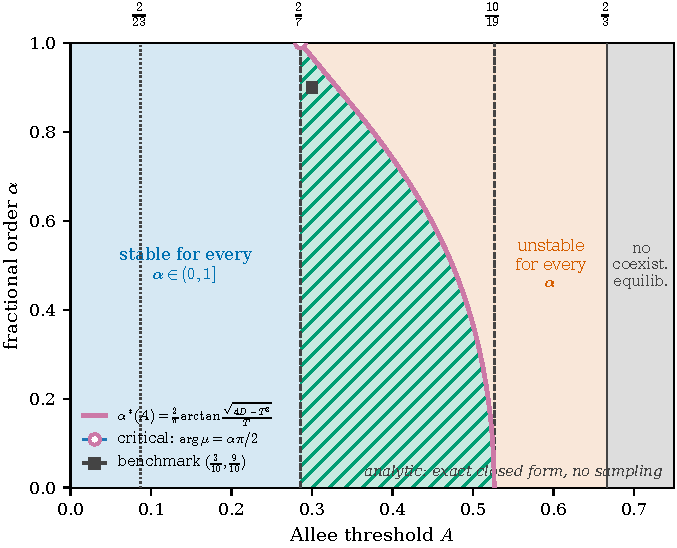
\includegraphics[width=0.65\textwidth]{fig02_stability_atlas.pdf}
\caption{{The benchmark} 
 atlas of Theorem~\ref{thm:atlas} from the closed form Equation~\eqref{eq:alphastar};
landmarks at $2/23$, $2/7$, $10/19$, $2/3$. Hatched: the region $\mathcal{W}$ of
Corollary~\ref{cor:wedge}, where $E^{*}$ is stable and the memoryless map is unstable for
every $\varepsilon>0$. Open circle: the critical point of Proposition~\ref{prop:critical} (i).
{{Analytic content.}
}}
\label{fig:atlas}
\end{figure}

\begin{Remark}[the benchmark point]\label{rem:baseline}
At $A=3/10$ one gets the exact values $T=1/24$, \linebreak  $D=11/60$, $\Delta=-2107/2880<0$, so case
(d) applies with
\[
  \upmu_{\pm} = \tfrac{1}{48} \pm i\,\tfrac{1}{2}\sqrt{\tfrac{2107}{2880}},
  \qquad \alpha^{*}(3/10)=0.969012276152\ldots
\]

In particular $\Real\upmu=1/48>0$: classical linear intuition reads this equilibrium as
unstable. Since the benchmark order is $\alpha=9/10<\alpha^{*}(3/10)$, the Caputo
equilibrium is in fact locally asymptotically stable. This single point is an illustration;
the content is the region.
\end{Remark}

Table~\ref{tab:scope} records the scope of every statement in the paper.

\begin{table}[H]
\caption{Scope of every statement in the paper: what it asserts, for which parameters, and
what kind of evidence supports it. ``Corroboration'' is finite-horizon numerics and is never
offered as proof.\label{tab:scope}}


\begin{adjustwidth}{-\extralength}{0cm}
%\centering %% If there is a figure in wide page, please release command \centering, for Table, ``\textwidth" should be ``\fulllength"
\footnotesize
\begin{tabularx}{\fulllength}{cCCC}
\toprule
\textbf{Statement} & \textbf{Parameter Scope} & \textbf{What is Asserted} & \textbf{Evidence} \\
\midrule
Theorems~\ref{thm:general} and \ref{thm:boundary} & whole family & closed-form equilibria, $(T,D)$ reduction & theorem; symbolic check \\
\midrule
Theorem~\ref{thm:classification} and Proposition~\ref{prop:critical} & whole family & Matignon classification; what the boundaries decide & theorem \\
\midrule
Theorem~\ref{thm:general-atlas}, Corollary~\ref{cor:open} & every set with $c_{T}<0$ (case (d)~otherwise) & six-row atlas, $\alpha^{*}$ strictly decreasing, open in parameter space & theorem; symbolic check \\
\midrule
Theorems~\ref{thm:atlas} and \ref{thm:monotone} & benchmark & rational breakpoints, explicit $\alpha^{*}$ & theorem; machine audit (Section~\ref{sec:certificates}) \\
\midrule
Theorem~\ref{thm:inversion}, Proposition~\ref{prop:onestep} & any equilibrium meeting (i)--(ii) & memoryless maps invert the verdict & theorem \\
\midrule
Corollaries~\ref{cor:wedge} and~\ref{cor:general-wedge} & benchmark/every set with $c_{T}<0$ & explicit region of inversion & theorem \\
\midrule
Theorem~\ref{thm:gl-implicit}, Proposition~\ref{prop:gl-explicit} & linear test equation, every $\upmu$ & Gr\"unwald--Letnikov schemes are verdict-faithful & theorem (Appendix~\ref{app:proofs}) \\
\midrule
Section~\ref{sec:global}, Proposition~\ref{prop:basins} & whole family & positivity, extinction strip, ultimate bound, global existence; what is not proved & theorem \\
\midrule
Section~\ref{sec:numerics} & benchmark, Sets II--III, random~ensemble & finite-horizon trajectories, convergence near $\alpha^{*}$ & corroboration only \\
\bottomrule
\end{tabularx}
\end{adjustwidth}
\end{table}

%=====================================================================
\section{Step-Size-Independent Verdict Inversion}\label{sec:inversion}
%=====================================================================

\textls[-15]{We now make precise the memoryless-surrogate failure described in the introduction, and
then place it in the dichotomy it belongs to. The object of Section~\ref{sec:memoryless} is a
discrete map that discards the fractional history; it is not proposed as an integrator for
Equation~\eqref{eq:model}. Proper fractional schemes retain the history, and their stability theory is
developed \cite{Lubich1986,Cermak2013,Garrappa2010,CressonSzafranska2017};
Section~\ref{sec:faithful} proves what the two simplest of them do on the same problem. One
terminology point: fast solvers that approximate the fractional kernel by a sum of
exponentials and carry the history through an augmented state
\cite{BaffetHesthaven2017,Jiang2017} store no explicit trajectory history and are sometimes
described as memory-free. They remain approximations of the nonlocal equation and are not the
object studied here; our use of ``memoryless'' is strict, the map $I+\varepsilon f$
containing no representation of the history whatsoever.}

\subsection{The Memoryless Map}\label{sec:memoryless}

\begin{Definition}[memoryless forward-Euler surrogate]\label{def:surrogate}
For $\varepsilon>0$ let $F_{\varepsilon}:\Omega\to\Rn^{2}$,
$F_{\varepsilon}(z)=z+\varepsilon f(z)$, with $f$ the right-hand side of Equation~\eqref{eq:model}
and $\Omega$ the open half-plane Equation~\eqref{eq:Omega} on which $f$ is defined. Every
equilibrium of Equation~\eqref{eq:model} is a fixed point of $F_{\varepsilon}$, with multiplier
spectrum $\{1+\varepsilon\upmu:\upmu\in\spec Df\}$. Since every coexistence equilibrium
considered below lies in the interior of $\Omega$ and $F_{\varepsilon}(z^{*})=z^{*}$,
continuity gives, for each fixed $\varepsilon>0$, a neighborhood of $z^{*}$ on which the
map and its iterates are well defined, at least until an orbit leaves that neighborhood;
the instability statements below are local, and no global invariance of $\Omega$ under
$F_{\varepsilon}$ is asserted.
\end{Definition}

$F_{\varepsilon}$ is memoryless: it uses only the current state. That is exactly what
disqualifies it as an approximation of a Caputo system, and exactly what makes the following
identity bite.

\begin{Lemma}[Euler multiplier identity]\label{lem:multiplier}
Let $\upmu\in\Cn$ and $\varepsilon>0$, and put $\lambda=1+\varepsilon\upmu$. Then
\begin{equation}\label{eq:identity}
  |\lambda|^{2}-1 \;=\; 2\varepsilon\Real\upmu+\varepsilon^{2}|\upmu|^{2}.
\end{equation}

Consequently $\Real\upmu>0$ implies $|\lambda|>1$ for \emph{every} $\varepsilon>0$.
\end{Lemma}

\begin{proof}
Write $\upmu=\rho+i\sigma$; then
$|\lambda|^{2}=(1+\varepsilon\rho)^{2}+\varepsilon^{2}\sigma^{2}
=1+2\varepsilon\rho+\varepsilon^{2}(\rho^{2}+\sigma^{2})$, which is~Equation~\eqref{eq:identity}. If
$\rho>0$ both terms on the right are positive for $\varepsilon>0$.
\end{proof}

\begin{Theorem}[memoryless-surrogate verdict inversion]\label{thm:inversion}
\textls[-15]{Let $z^{*}$ be an equilibrium of the commensurate Caputo system Equation~\eqref{eq:model} of order
$0<\alpha<1$, with Jacobian $J=Df(z^{*})$. Assume}
\begin{enumerate}[label=(\roman*),leftmargin=*,itemsep=1pt]
\item \emph{every} eigenvalue satisfies the sector condition:
      $\spec(J)\subset\{\upmu\neq0:|\arg\upmu|>\alpha\pi/2\}$;
\item \emph{some} eigenvalue has a positive real part.
\end{enumerate}

Then, $z^{*}$ is locally asymptotically stable for Equation~\eqref{eq:model}, while the fixed point of
$F_{\varepsilon}$ is linearly unstable for every $\varepsilon>0$.
\end{Theorem}

\begin{proof}
Hypothesis (i) is exactly the spectral hypothesis of the nonlinear fractional linearization
theorem \cite{Cong2016}, valid for $0<\alpha<1$, which gives local asymptotic stability. For
(ii), let $\upmu\in\spec(J)$ with $\Real\upmu>0$; then $1+\varepsilon\upmu$ is an eigenvalue of
$DF_{\varepsilon}(z^{*})=I+\varepsilon J$, and Lemma~\ref{lem:multiplier} gives
$|1+\varepsilon\upmu|>1$ for every $\varepsilon>0$, so a multiplier lies outside the closed
unit disc, and the fixed point is linearly unstable. The two conclusions are compatible
because the sector $\{|\arg\upmu|>\alpha\pi/2\}$ meets the open right half-plane whenever
$\alpha<1$.
\end{proof}

\begin{Remark}[the quantifiers are not interchangeable]\label{rem:quantifiers}
Hypothesis (i) is about the \emph{whole} spectrum, and hypothesis (ii) is about \emph{one}
eigenvalue, and neither can be relaxed to the other. Weakening (i) to ``some eigenvalue lies
outside the sector'' would be false: the Jacobian $\diag(\tfrac{1}{48}+\tfrac{i}{2},\,
\tfrac{1}{10})$ at $\alpha=9/10$ has a first eigenvalue outside the forbidden sector with
positive real part, yet its second eigenvalue is real and positive and destabilizes the
equilibrium. Conversely, (ii) genuinely needs only one eigenvalue, because a single
multiplier outside the unit disc suffices for linear instability of a map. A regression
fixture pins in both directions.
\end{Remark}

The identity is elementary; the point is what it excludes. No choice of $\varepsilon$
recovers the correct verdict, so the failure cannot be diagnosed or repaired by a
convergence study. It is not that the surrogate is inaccurate at coarse steps and accurate
at fine ones; it is qualitatively wrong at all of them.

\begin{Corollary}[a full region of guaranteed inversion]\label{cor:wedge}
For the benchmark Equation~\eqref{eq:benchmark}, let
\[
  \mathcal{W} \;=\; \Bigl\{(A,\alpha) \;:\; \tfrac{2}{7}<A<\tfrac{10}{19},
    \;\; 0<\alpha<\alpha^{*}(A) \Bigr\}.
\]

For every $(A,\alpha)\in\mathcal{W}$ the coexistence equilibrium $E^{*}$ of
Equation~\eqref{eq:model} is locally asymptotically stable, while for every $\varepsilon>0$ the
corresponding fixed point of $F_{\varepsilon}$ is linearly unstable. $\mathcal{W}$ is
nonempty with nonempty interior, and $\alpha^{*}$ is strictly decreasing across it from $1$
to $0$.
\end{Corollary}

\begin{proof}
On $2/7<A<10/19$, Theorem~\ref{thm:atlas} gives $\Delta(A)<0$ and $T(A)>0$, so the spectrum
is the conjugate pair $\rho\pm i\sigma$ with $\rho=T(A)/2>0$ and $\sigma>0$. Both eigenvalues
have the same modulus of argument, so for the $\alpha<\alpha^{*}(A)$ hypothesis (i) of
Theorem~\ref{thm:inversion} holds for the {{entire}} spectrum, by
Theorem~\ref{thm:classification} (d), and hypothesis (ii) holds because $\rho>0$. This is
exactly why the corollary is not caught by Remark~\ref{rem:quantifiers}: for a conjugate
pair, ``some eigenvalue'' and ``every eigenvalue'' coincide. Nonemptiness and the endpoint
limits are Theorem~\ref{thm:monotone}.
\end{proof}

\begin{Corollary}[inversion region for every parameter set with $c_{T}<0$]\label{cor:general-wedge}
Let the parameter set satisfy $ea>mh$, $q<K$, and $c_{T}<0$, and let $\mathcal{W}$ be the
region Equation~\eqref{eq:W-general}. For every $(A,\alpha)\in\mathcal{W}$ the coexistence
equilibrium is locally asymptotically stable for Equation~\eqref{eq:model}, while the fixed point of
$F_{\varepsilon}$ is linearly unstable for every $\varepsilon>0$.
\end{Corollary}

\begin{proof}
On $(A_{T},A_{2})$ the spectrum is a complex pair with $\Real\upmu=T/2>0$
(Theorem~\ref{thm:general-atlas} (b)), and for $\alpha<\alpha^{*}(A)$ both eigenvalues satisfy
the sector condition (Theorem~\ref{thm:classification} (d)); Theorem~\ref{thm:inversion}
applies.
\end{proof}

Figure~\ref{fig:spectral} shows the mechanism at the benchmark point.

\begin{figure}[H]
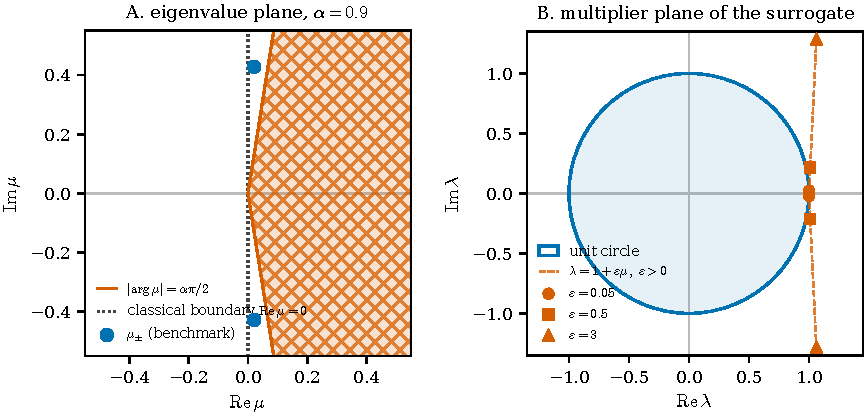
\includegraphics[width=0.85\textwidth]{fig03_spectral_geometry.pdf}
\caption{(\textbf{A}) {eigenvalue} plane at $\alpha=0.9$; the hatched sector, not the right half-plane,
is the Caputo-unstable set, and the benchmark pair lies outside it although
$\Real\upmu=1/48>0$. (\textbf{B}) multiplier plane of $F_{\varepsilon}$; by Equation~\eqref{eq:identity}
the image curve $\varepsilon\mapsto1+\varepsilon\upmu$ leaves the unit disc at once and never
returns. {{Analytic content.}}}
\label{fig:spectral}
\end{figure}

\subsection{History-Retaining Schemes Are Verdict-Faithful}\label{sec:faithful}

Theorem~\ref{thm:inversion} concerns the memoryless map. The natural question is what a
scheme that keeps the history does on the same problem, and the answer is a dichotomy.
Consider the scalar test equation
\begin{equation}\label{eq:test}
  \Dc{\alpha}y=\upmu y,\qquad y(0)=y_{0},\qquad 0<\alpha<1,\quad \upmu\in\Cn\setminus\{0\},
\end{equation}
whose solution $y(t)=y_{0}\Eml{\alpha}(\upmu t^{\alpha})$ tends to $0$ iff
$|\arg\upmu|>\alpha\pi/2$, in which case
\linebreak  $y(t)=-y_{0}\bigl(\upmu\,\Gamma(1-\alpha)\,t^{\alpha}\bigr)^{-1}(1+o(1))$
\cite{Podlubny1999}. When $\Delta\neq0$ the linearization of each scheme below at an
equilibrium of Equation~\eqref{eq:model} decouples into two copies of Equation~\eqref{eq:test} with
$\upmu=\upmu_{\pm}$, so Equation~\eqref{eq:test} carries the linear stability verdict of the scheme exactly
as it does for the continuous system.

Let $\omega_{j}=(-1)^{j}\binom{\alpha}{j}$, so that $\sum_{j\ge0}\omega_{j}\xi^{j}=(1-\xi)^{\alpha}$,
and let $u_{n}=y_{n}-y_{0}$. The {{implicit}} and {{explicit}} Gr\"unwald--Letnikov
schemes with step $h>0$ are
\begin{equation}\label{eq:gl}
  h^{-\alpha}\sum_{j=0}^{n}\omega_{j}u_{n-j}=f(y_{n})
  \qquad\text{and}\qquad
  h^{-\alpha}\sum_{j=0}^{n}\omega_{j}u_{n-j}=f(y_{n-1}),\qquad n\ge1,
\end{equation}
the convolution quadratures of Lubich \cite{Lubich1986} generated by the backward-difference
symbol. Both are first-order consistent for the Caputo problem \cite{Lubich1986,Garrappa2018},
and both sum over the whole history at every step. Put $z=h^{\alpha}\upmu$.

\begin{Theorem}[the implicit Gr\"unwald--Letnikov scheme is verdict-faithful for every step]
\label{thm:gl-implicit}
Apply the implicit scheme Equation~\eqref{eq:gl} to Equation~\eqref{eq:test}.
\begin{enumerate}[label=(\alph*),leftmargin=*,itemsep=1pt]
\item If $|\arg\upmu|>\alpha\pi/2$, then for every $h>0$ the scheme is well defined,
      $y_{n}\to0$, and
      \[
        y_{n}\;=\;-\frac{y_{0}}{\upmu\,\Gamma(1-\alpha)\,t_{n}^{\alpha}}\bigl(1+o(1)\bigr),
        \qquad t_{n}=nh,
      \]
      the same leading asymptotics as the exact solution, at every step size.
\item If $|\arg\upmu|<\alpha\pi/2$ and
      $0<h<h_{1}(\upmu,\alpha):=2\cos(\arg\upmu/\alpha)\,|\upmu|^{-1/\alpha}$ with
      $h^{\alpha}\upmu\neq1$, then $|y_{n}|\to\infty$ at an exponential rate.
\end{enumerate}

In particular, on the region $\mathcal{W}$ of Corollaries~\ref{cor:wedge} and
\ref{cor:general-wedge} the implicit scheme returns the Caputo verdict at every step size,
while the memoryless map returns the opposite verdict at every step size.
\end{Theorem}

\begin{Proposition}[the explicit scheme is verdict-faithful for every sufficiently small step]
\label{prop:gl-explicit}
Apply the explicit scheme Equation~\eqref{eq:gl} to Equation~\eqref{eq:test}. If $|\arg\upmu|>\alpha\pi/2$ there
is $h_{0}(\upmu,\alpha)>0$ such that $y_{n}\to0$ for every $0<h<h_{0}$; if
$|\arg\upmu|<\alpha\pi/2$ there is $h_{0}>0$ such that $|y_{n}|\to\infty$ for every
$0<h<h_{0}$. The threshold is read off the exact boundary locus
$\theta\mapsto(1-e^{i\theta})^{\alpha}e^{-i\theta}$ of the scheme's stability set; at the
benchmark eigenvalue and $\alpha=9/10$ it is $h_{0}=0.505\ldots$.
\end{Proposition}

\begin{Proposition}[every consistent memoryless one-step method inverts the verdict for small steps]
\label{prop:onestep}
Let $R$ be the stability function of a consistent one-step method for an ordinary differential
equations, so that $R(w)=1+w+O(w^{2})$ as $w\to0$ \emph{\cite{HairerWanner1996}}; applied
memorylessly to Equation~\eqref{eq:model}, the method has multipliers $R(\varepsilon\upmu)$ at an
equilibrium. If $\Real\upmu>0$ there is $\varepsilon_{0}>0$ such that $|R(\varepsilon\upmu)|>1$
for all $0<\varepsilon<\varepsilon_{0}$. For the forward-Euler map $R(w)=1+w$ one may take
$\varepsilon_{0}=\infty$ (Lemma~\ref{lem:multiplier}).
\end{Proposition}

The proofs are in Appendix~\ref{app:proofs}. The one for Theorem~\ref{thm:gl-implicit} is a
generating-function argument on the closed unit disc in the spirit of \cite{Lubich1986}, with
the asymptotics supplied by singularity analysis \cite{FlajoletSedgewick2009};
Section~\ref{sec:num-schemes} corroborates both statements
numerically, on the test equation and on the nonlinear benchmark.

\begin{Remark}[what the dichotomy says, and what it does not]\label{rem:dichotomy}
\textls[-15]{(i) The two families are separated by a structural property, not by accuracy. A memoryless
one-step method sees the equilibrium through $R(\varepsilon\upmu)$, and consistency forces
$|R(\varepsilon\upmu)|^{2}=1+2\varepsilon\Real\upmu+O(\varepsilon^{2})$: the sign of $\Real\upmu$
decides the small-step verdict, and the method cannot know $\alpha$. A history-retaining
scheme sees it through the symbol $(1-\xi)^{\alpha}$, whose values on the closed unit disc
fill a bounded lens inside the sector $|\arg w|\le\alpha\pi/2$ that also governs the
continuous equation; the stability set of the implicit scheme is exactly the complement of
that lens, and that of the explicit scheme is a bounded set tangent to the sector boundary at
the origin (Section~\ref{sec:num-schemes}). (ii) A memoryless method can return the right
verdict at isolated step sizes by coincidence: the stability region of the classical
fourth-order Runge--Kutta method contains a neighborhood of the open segment
$\{iy:0<|y|<2\sqrt2\}$ of the imaginary axis and therefore enters the open right half-plane,
so a ray $\arg w=\arg\upmu$ very close to the imaginary axis can cross it.
Proposition~\ref{prop:onestep} says that no such coincidence survives mesh refinement. (iii)
The Diethelm--Ford--Freed predictor--corrector method used in Section~\ref{sec:numerics}
also retains the history; its linear stability set is bounded and was computed by Garrappa
\emph{\cite{Garrappa2010}}. We prove no small-step statement for it here and rely on its convergence
theory \emph{\cite{Diethelm2002}} and on the corroboration of Section~\ref{sec:num-schemes}. (iv)
Nothing in this section is a statement about Gr\"unwald--Letnikov or predictor--corrector
schemes being unreliable; the point is the converse, that carrying the memory is what makes a
scheme able to see fractional stabilization at all.}
\end{Remark}

%=====================================================================
\section{\textls[-15]{Global Behavior: Uniform Ultimate Bound, Global Existence, Extinction}}\label{sec:global}

\textls[-15]{The results of this section are included for completeness: they are proved with standard
tools (fractional first-contact arguments, the scalar Caputo comparison principle, and one
linear functional), we claim no novelty of method, and their role is to place the local
classification of Section~\ref{sec:atlas} inside a global picture. What they do not give is
stated in Proposition~\ref{prop:basins}. Everything up to Corollary~\ref{cor:global} is
established on the maximal interval $[0,T_{\max})$ only.}

We use one standard tool, stated for reference.

\begin{Lemma}[scalar Caputo comparison]\label{lem:comparison}
Let $0<\alpha\le1$ and $c>0$. Let $g$ be nonnegative on $[0,T)$ and lie on every compact
subinterval, in the regularity class of Proposition~\ref{prop:local}---continuous, \linebreak  $C^{1}$
away from $0$ with $g'(t)=O(t^{\alpha-1})$, so that the Caputo derivative exists pointwise---and suppose $\Dc{\alpha}g(t)\le-c\,g(t)$ on $(0,T)$. Then,
$g(t)\le g(0)\,\Eml{\alpha}(-c\,t^{\alpha})$ on $[0,T)$, and in particular
$g(t)\to0$ as $t\to\infty$ when $T=\infty$. More generally, for $g$ in the same class, if
$\Dc{\alpha}g\le-c\,g+\phi(t)$ with $\phi$ continuous, then
\begin{equation}\label{eq:resolvent}
  g(t)\;\le\; g(0)\Eml{\alpha}(-c\,t^{\alpha})
    + \int_{0}^{t}(t-s)^{\alpha-1}\Emlt{\alpha}{\alpha}\!\left(-c\,(t-s)^{\alpha}\right)\phi(s)\,ds,
\end{equation}
the kernel being nonnegative, with
\begin{equation}\label{eq:kernelmass}
  \int_{0}^{t}\tau^{\alpha-1}\Emlt{\alpha}{\alpha}(-c\,\tau^{\alpha})\,d\tau
  \;=\;\frac{1-\Eml{\alpha}(-c\,t^{\alpha})}{c}\;\le\;\frac{1}{c}.
\end{equation}
\end{Lemma}

\begin{proof}
Both are standard; see (Chapter~7, \cite{Diethelm2010}) for the comparison principle and the
Mittag-Leffler resolvent representation of the scalar linear Caputo equation, and
\cite{Podlubny1999} for Equation~\eqref{eq:kernelmass}, which follows by termwise integration of the
series for $\Emlt{\alpha}{\alpha}$.
\end{proof}

\subsection{A Uniform Ultimate Bound on the Maximal Interval}

\begin{Theorem}[uniform ultimate bound]\label{thm:bounded}
Let the initial data be nonnegative and let $[0,T_{\max})$ be the maximal interval of
Proposition~\ref{prop:local}. Put $Q(x)=P(x)+mx$ and
\begin{equation}\label{eq:C}
  C \;=\; e\max_{x\ge0}Q(x),
\end{equation}
which is finite and nonnegative. Then, on $[0,T_{\max})$,

\[
  W(t)=e\,x(t)+y(t)\;\le\; W(0)\,\Eml{\alpha}(-m\,t^{\alpha})
      +\frac{C}{m}\bigl(1-\Eml{\alpha}(-m\,t^{\alpha})\bigr)
  \;\le\;\max\Bigl\{W(0),\frac{C}{m}\Bigr\}.
\]
\end{Theorem}

\begin{proof}
$Q$ is a cubic with leading coefficient $-r/(AK)<0$, so $Q(x)\to-\infty$ as $x\to\infty$ and
the maximum over $[0,\infty)$ is attained and finite; $Q(0)=0$ gives $C\ge0$. By
Theorem~\ref{thm:positive-invariance}, $x,y\ge0$ on $[0,T_{\max})$. Substituting $y=W-ex$ in
the exact cancellation Equation~\eqref{eq:W},
\[
  \Dc{\alpha}W \;=\; e\,P(x)-m\,y \;=\; -m\,W+e\bigl(P(x)+mx\bigr)\;\le\;-m\,W+C,
\]
and Lemma~\ref{lem:comparison} applied to $W$ gives the displayed estimate; the final bound
follows because a convex combination of $W(0)$ and $C/m$ never exceeds their maximum.
\end{proof}



\begin{Corollary}[global existence]\label{cor:global}
For every nonnegative initial condition, $T_{\max}=\infty$: the solution of Equation~\eqref{eq:model}
exists for all $t\ge0$, and consequently
\[
  \limsup_{t\to\infty}\bigl(e\,x(t)+y(t)\bigr)\;\le\;\frac{C}{m},
\]
a bound \emph{independent of the initial condition}.
\end{Corollary}

\begin{proof}
\textls[-15]{By Theorem~\ref{thm:bounded} and positivity, $x\le W/e$ and $y\le W\le\max\{W(0),C/m\}$
stay in a fixed compact subset of $\Omega$ on $[0,T_{\max})$, which excludes the blow-up
horn of the continuation alternative for Caputo equations with locally Lipschitz right-hand
side (Chapter 6, \cite{Diethelm2010}), \cite{CarvalhoFehlberg2018}; hence $T_{\max}=\infty$. The
$\limsup$ follows from Theorem~\ref{thm:bounded} since $\Eml{\alpha}(-mt^{\alpha})\to0$.}
\end{proof}

\begin{Corollary}[the invariance statements hold for all time]\label{cor:promote}
For every nonnegative initial condition and every $t\ge0$: $x(t)\ge0$, $y(t)\ge0$,
$x(t)\le\max\{K,x(0)\}$, and $x(t)\le x_{0}$ whenever $0<x_{0}=x(0)<A$. Moreover
$\limsup_{t\to\infty}\bigl(ex(t)+y(t)\bigr)\le C/m$.
\end{Corollary}

\begin{proof}
Theorem~\ref{thm:positive-invariance} gives all four bounds on $[0,T_{\max})$, and
Corollary~\ref{cor:global} gives $T_{\max}=\infty$; the $\limsup$ is the last statement of
that corollary.
\end{proof}

\begin{Remark}[uniform ultimate level]\label{rem:ultimate-level}
\textls[-25]{For every $\eta>0$ and every nonnegative initial state there, is a time after which
$ex(t)+y(t)\le C/m+\eta$, and the level $C/m$ does not involve the initial state; for the
benchmark $C/m=\tfrac{910+103\sqrt{103}}{1350}=1.4483\ldots$ (Figure~\ref{fig:dissipative}).
We do not call the region an absorbing set, since an autonomous Caputo equation need not
generate a semiflow (Remark~\ref{rem:nocross}); $W$ bounds $ex+y$ and nothing sharper, and
an initially over-capacity prey population is not asserted to fall below $K$.}
\end{Remark}

\begin{figure}[H]
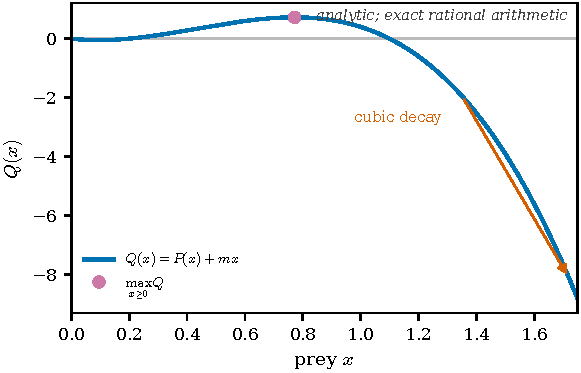
\includegraphics[width=0.5\textwidth]{fig08_dissipative.pdf}
\caption{\textls[-35]{Why the uniform ultimate level carries no memory of the initial condition: the
cubic \linebreak  $Q(x)=P(x)+mx$ has a finite maximum on $[0,\infty)$, attained for the benchmark at
$x=\tfrac{13+\sqrt{103}}{30}$ with \linebreak  $C/m=\tfrac{910+103\sqrt{103}}{1350}=1.44839\ldots$, a
constant of the vector field alone. {{Analytic content; no trajectory integrated.}}}}
\label{fig:dissipative}
\end{figure}

\subsection{The Extinction Strip}

\begin{Theorem}[extinction of the prey]\label{thm:extinction}
Let $0<A<K$, let the initial data be nonnegative, and let $x_{0}:=x(0)$ satisfy
$0<x_{0}<A$ (for $x_{0}=0$, $x\equiv0$ by uniqueness). Put
\begin{equation}\label{eq:c}
  c \;=\; r\Bigl(1-\frac{x_{0}}{K}\Bigr)\Bigl(1-\frac{x_{0}}{A}\Bigr) \;>\;0 .
\end{equation}

Then, $x(t)\le x_{0}\,\Eml{\alpha}(-c\,t^{\alpha})\to0$ for every $\alpha\in(0,1]$.
\end{Theorem}

\begin{proof}
By Corollary~\ref{cor:promote} the solution satisfies $0\le x(t)\le x_{0}$ for all
$t\ge0$, so it remains in the strip. On $[0,x_{0}]$ we have, writing
$P(x)=-r\,x(1-x/K)(1-x/A)$,
\[
  P(x) \;=\; -r\,x\Bigl(1-\frac{x}{K}\Bigr)\Bigl(1-\frac{x}{A}\Bigr)
        \;\le\; -c\,x,
\]
because $1-x/K\ge1-x_{0}/K>0$ and $1-x/A\ge1-x_{0}/A>0$ there. Predation is nonpositive
in the prey equation for $y\ge0$, so $\Dc{\alpha}x\le P(x)\le-c\,x$ on the strip, and
Lemma~\ref{lem:comparison} gives the stated Mittag-Leffler envelope.
\end{proof}

\begin{Lemma}[vanishing forcing]\label{lem:vanishing}
Let $0<\alpha\le1$, $c>0$, and let $g\ge0$ lie in the class of Lemma~\ref{lem:comparison} on
$[0,\infty)$ with $\Dc{\alpha}g\le-c\,g+\phi(t)$, where $\phi$ is continuous, nonnegative, and
$\phi(t)\to0$. Then $g(t)\to0$.
\end{Lemma}

\begin{proof}
By Equation~\eqref{eq:resolvent} it suffices to treat the convolution term. Given $\eta>0$ choose $S$
with $\phi\le\eta$ on $[S,\infty)$ and split at $S$: by nonnegativity of the kernel and
Equation~\eqref{eq:kernelmass} the part over $[S,t]$ is at most $\eta/c$, while the part over $[0,S]$
is at most $\sup_{[0,S]}\phi\int_{t-S}^{t}\tau^{\alpha-1}\Emlt{\alpha}{\alpha}(-c\tau^{\alpha})\,d\tau$,
which tends to $0$ as the tail of a convergent integral. Hence,
$\limsup_{t\to\infty}g(t)\le\eta/c$ for every $\eta>0$.
\end{proof}

\begin{Theorem}[extinction of the predator follows]\label{thm:predator}
Under the hypotheses of Theorem~\ref{thm:extinction}, $y(t)\to0$ as well.
\end{Theorem}

\begin{proof}
Let $W=e\,x+y$. The predation terms cancel exactly:
\begin{equation}\label{eq:W}
  \Dc{\alpha}W \;=\; e\,P(x)-m\,y \;=\; -m\,W + e\,P(x) + m\,e\,x .
\end{equation}

Put $\phi(t)=|e\,P(x(t))+m\,e\,x(t)|$, which is continuous and nonnegative. By
Theorem~\ref{thm:extinction} $x(t)\to0$, and $P$ is continuous with $P(0)=0$, so
$\phi(t)\to0$. Since $\Dc{\alpha}W\le-mW+\phi$, Lemma~\ref{lem:vanishing} gives
$W(t)\to0$, and as $x,y\ge0$ with $e>0$ this forces $y(t)\to0$.
\end{proof}

\begin{Proposition}[what is and is not proved about long-time behavior]\label{prop:basins}
Let $ea>mh$ and $0<A<q<K$.
\begin{enumerate}[label=(\roman*),leftmargin=*,itemsep=1pt]
\item The strip $\{0\le x_{0}<A,\ y_{0}\ge0\}$ is contained in the basin of attraction of
      $E_{0}$ \linebreak  (Theorems~\ref{thm:extinction} and \ref{thm:predator}).
\item On the predator-free face the strip is sharp: if $y_{0}=0$ and $A<x_{0}<K$, then
      $x(t)\ge x_{0}>A$ for all $t\ge0$, so no prey level above $A$ leads to extinction
      there. Consequently, the strip cannot be widened in $x_{0}$ uniformly in $y_{0}$.
\item Wherever $E^{*}$ is Matignon-stable, $E_{0}$ and $E^{*}$ are both locally
      asymptotically stable: equilibrium bistability. The boundary between their basins is
      not characterized in this paper. With $y_{0}>0$ the extinction basin may exceed the
      strip, since predation can drive the prey below $A$, and by how much is not determined
      here.
\item No global asymptotic stability statement for $E^{*}$ is made, under any condition, and
      the set of asymptotic outcomes once $E^{*}$ is Matignon-unstable is not resolved: among
      the equilibria classified here only $E_{0}$ is then locally asymptotically stable, and
      nothing more is asserted.
\end{enumerate}
\end{Proposition}

\begin{proof}
(i) restates the two theorems. (ii): the face $y\equiv0$ is invariant, by $f_{2}(x,0)=0$ and
uniqueness, and on it the prey obeys $\Dc{\alpha}x=P(x)$ with $P>0$ on $(A,K)$. Suppose
$x$ first reaches $x_{0}-\delta$, with $0<\delta<x_{0}-A$, at some $t_{*}>0$. Then,
$x(t_{*})<x(0)$ is the minimum of $x$ over $[0,t_{*}]$, so Lemma~\ref{lem:extremum} gives
$\Dc{\alpha}x(t_{*})<0$, whereas $P(x(t_{*}))=P(x_{0}-\delta)>0$: a contradiction. Letting
$\delta\downarrow0$ gives $x\ge x_{0}$ (for $\alpha=1$ the classical first-hit argument
applies). (iii) is Theorem~\ref{thm:boundary} together with Theorem~\ref{thm:classification},
and (iv) is a statement about what is not proved.
\end{proof}

%=====================================================================
\section{Computer-Assisted Verification}\label{sec:certificates}
%=====================================================================

The theorems above are analytic and do not depend on the certificate layer. Independently
of them, the proof objects provide audits of selected algebraic identities, benchmark
constants, boundary points, and finite parameter boxes, re-derived by a separate program from
the model definition and each object's recorded parameters. Each object is described below
by the exact subclaim and parameter scope; its checker re-derives. A box object is uniform
over the box it declares; a finite family of such objects is a regression audit of the
theorem on those boxes, not a machine proof of the continuum theorem, and no such coverage
is claimed. The purpose is not to replace the proofs but to let a reader check the
arithmetic without trusting the authors---and the scope statement of each object is part
of that contract.

\subsection*{What Is Exact, What Is Enclosed}

The distinction that organizes the implementation is between claims that are algebraic and
claims that are not.

{{Algebraic claims are computed in exact rational arithmetic.}
} All parameters are exact
rationals and the coexistence equilibrium has the closed-form Equation~\eqref{eq:Estar}, so $T$, $D$
and $\Delta$ are exact rationals: at the benchmark, exactly $1/24$, $11/60$, and
$-2107/2880$. This matters for the critical cases. At $A=2/7$ the trace vanishes
{{exactly}}, which is what makes Theorem~\ref{thm:classification} (b) decidable and lets
the checker report ``stable'' for $\alpha<1$ and ``critical'' at $\alpha=1$ rather than
guessing. Likewise, at $A=2/3$ the second eigenvalue of $E_{A}$ vanishes exactly, which is
what licenses the verdict ``critical'' there, and $P(K)=0$ identically. A floating-point or
interval computation could only ever report an interval containing zero, which is a strictly
weaker statement: such an interval also admits nonzero values of either sign, so it cannot
decide a case whose entire content is that a quantity is exactly zero.

\textls[-15]{{{Non-algebraic claims are enclosed with certified interval arithmetic.}} Interval
endpoints are exact rationals; the field operations are exact rational arithmetic, with
endpoints rounded {{outward}} once they grow beyond a fixed size bound, so an enclosure
can only widen. The transcendental functions actually needed---$\sqrt{\cdot}$,
$\arctan$, $\pi$, and real powers---are enclosed by the Arb library, whose contract is
that every returned ball provably contains the exact result.}

The inventory of objects, the integrity properties enforced on them (a parameter lock and
manifest completeness), the semantics of a certificate that carries an interval of
parameters, and the second, independent checker are available from the corresponding author
on request. Two facts about them are worth stating here. Every interval-valued object is required
to contain the entire equilibrium curve over the interval it declares, so that it certifies
what its parameters say; and the second checker, built on a different arithmetic library and
a different formulation of the sector test, contradicts the first nowhere, returning
{{undecided}} exactly on the five objects whose content is an algebraic zero that binary
interval arithmetic cannot decide.

%=====================================================================
\section{Numerical Corroboration}\label{sec:numerics}
%=====================================================================

The figures and tables in this section are numerical corroboration and not proof, and each
answers one theorem. Unless stated otherwise, they are produced with the Diethelm--Ford--Freed
predictor--corrector method (PECE) for Caputo equations \cite{Diethelm2002}, which carries
the full fractional memory; Section~\ref{sec:num-schemes} also uses the two
Gr\"unwald--Letnikov schemes Equation~\eqref{eq:gl}. The memoryless map of
Section~\ref{sec:inversion} appears only as the {{object under study}}; it is never used to
simulate Equation~\eqref{eq:model}.

The solver is self-tested before use against facts it cannot fake: at $\alpha=1$ it
reproduces $e^{-2}$ for $y'=-y$ to $1.1\times10^{-8}$; for $\Dc{\alpha}y=-y$ it reproduces
$\Eml{\alpha}(-1)$ to $3.7\times10^{-8}$ at $\alpha=0.5$ and $2.1\times10^{-9}$ at
$\alpha=0.9$; and the observed order of convergence under successive mesh halving is
$1.90$, $1.90$, $1.89$. Every panel below states its parameters, initial condition, and
mesh; machine-readable data for every plotted point ship with the figure sources.

\subsection{Crossing the Critical Order}\label{sec:num-crossing}



Nothing changes between the four columns of Figure~\ref{fig:crossing} except $\alpha$, and
the qualitative behavior flips where Theorem~\ref{thm:atlas} says it must.

\begin{figure}[H]
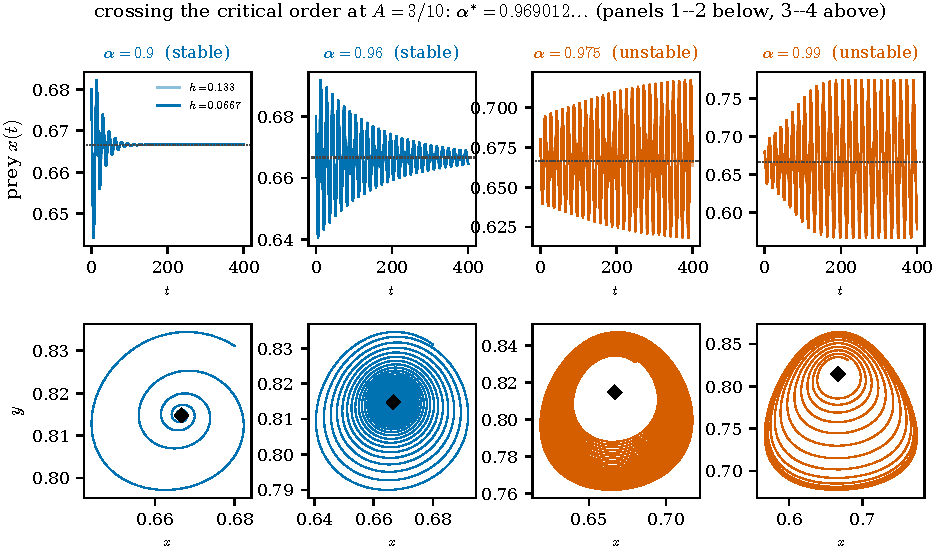
\includegraphics[width=0.85\textwidth]{figB_crossing_alpha_star.pdf}
\caption{Crossing $\alpha^{*}(3/10)=0.969012\ldots$ at the benchmark from $1.02\,E^{*}$,
$T=400$. Columns: $\alpha=0.90$, $0.96$ (Matignon-stable) and $0.975$, $0.99$
(Matignon-unstable); final-to-initial distance ratios $1.1\times10^{-3}$, $10^{-1}$, $1.5$,
$4.3$. (\textbf{Top}) prey time series at $n=3000$ and $6000$ overlaid, indistinguishable. (\textbf{Bottom})
{phase portraits}.%{{Corroboration of Theorems~\ref{thm:classification} and\ref{thm:atlas}, not proof.}}
}
\label{fig:crossing}
\end{figure}

\subsubsection*{{Convergence and Horizon Sensitivity Near the Critical Order}
}
Table~\ref{tab:convergence} records what a finite-horizon simulation can and cannot decide
close to $\alpha^{*}$. For $\alpha<\alpha^{*}$ the approach to $E^{*}$ is algebraic, like
$t^{-\alpha}$; for $\alpha>\alpha^{*}$ the departure is exponential with the linear rate
$\lambda_{\mathrm{lin}}=|\upmu|^{1/\alpha}\cos(\arg\upmu/\alpha)$, which vanishes exactly at
$\alpha^{*}$. Two facts follow from the table. The mesh is not the limiting factor: the
difference between the two finest meshes at $T=400$ is below $5\times10^{-4}$ for every
$\alpha$, and the observed order of convergence is $1.9$. The horizon is: at $T=400$ the
endpoint diagnostic is undecided for $|\alpha-\alpha^{*}|\lesssim0.006$, at $T=800$ for
$|\alpha-\alpha^{*}|\lesssim0.003$, and the undecided window shrinks with $T$ exactly as
$\lambda_{\mathrm{lin}}$ predicts. The endpoint map of Section~\ref{sec:num-maps} must be
read with this in mind: a cell classified ``transient'' near the curve $\alpha^{*}(A)$ is
the expected finite-horizon behavior, not evidence against the theorem.

\begin{table}[H]
\caption{{PECE} 
 at the benchmark $A=3/10$ from $1.02\,E^{*}$ near $\alpha^{*}=0.969012\ldots$:
Matignon verdict, linear rate $\lambda_{\mathrm{lin}}$, horizon $T$, finest mesh $n$,
distance ratio $r_{T}=\|z(T)-E^{*}\|/\|z(0)-E^{*}\|$ at the two finest meshes, mesh-to-mesh
difference, and endpoint class ($r_{T}<1/2$ decaying, $r_{T}>2$ growing, otherwise undecided
at this horizon). } % {{Corroboration.}}
\label{tab:convergence}

\begin{adjustwidth}{-\extralength}{0cm}
\small
		\begin{tabularx}{\fulllength}{RRLRRRRRRL}
\toprule
\boldmath{$\alpha$} & \boldmath{$\alpha-\alpha^{*}$} & \textbf{Matignon} & \boldmath{$10^{3}\lambda_{\mathrm{lin}}$} & \boldmath{$T$} & \boldmath{$n$} & \boldmath{$r_{T}$} & \boldmath{$r_{T}$} at \boldmath{$n/2$} & \textbf{Mesh Diff.} & \textbf{at} \boldmath{$T$} \\
\midrule
0.9000 & $-0.0690$ & stable & $-46.82$ & 400 & 16000 & 0.0011 & 0.0011 & $3\times10^{-10}$ & decaying \\
0.9500 & $-0.0190$ & stable & $-12.87$ & 400 & 16000 & 0.0067 & 0.0067 & $2\times10^{-6}$ & decaying \\
0.9600 & $-0.0090$ & stable & $-6.09$ & 400 & 16000 & 0.099 & 0.099 & $3\times10^{-5}$ & decaying \\
0.9650 & $-0.0040$ & stable & $-2.71$ & 400 & 16000 & 0.372 & 0.372 & $9\times10^{-5}$ & decaying \\
0.9680 & $-0.0010$ & stable & $-0.68$ & 400 & 16000 & 0.753 & 0.755 & $2\times10^{-4}$ & undecided \\
0.9690 & $-0.0000$ & stable & $-0.01$ & 400 & 16000 & 0.925 & 0.928 & $2\times10^{-4}$ & undecided \\
0.9695 & $+0.0005$ & unstable & $+0.33$ & 400 & 16000 & 1.02 & 1.02 & $2\times10^{-4}$ & undecided \\
0.9700 & $+0.0010$ & unstable & $+0.67$ & 400 & 16000 & 1.10 & 1.11 & $2\times10^{-4}$ & undecided \\
0.9720 & $+0.0030$ & unstable & $+2.02$ & 400 & 16000 & 1.37 & 1.38 & $3\times10^{-4}$ & undecided \\
0.9750 & $+0.0060$ & unstable & $+4.04$ & 400 & 16000 & 1.55 & 1.55 & $4\times10^{-4}$ & undecided \\
0.9900 & $+0.0210$ & unstable & $+14.13$ & 400 & 16000 & 4.30 & 4.31 & $4\times10^{-4}$ & growing \\
\midrule
0.9650 & $-0.0040$ & stable & $-2.71$ & 800 & 32000 & 0.120 & 0.120 & $6\times10^{-5}$ & decaying \\
0.9680 & $-0.0010$ & stable & $-0.68$ & 800 & 32000 & 0.514 & 0.515 & $2\times10^{-4}$ & undecided \\
0.9690 & $-0.0000$ & stable & $-0.01$ & 800 & 32000 & 0.768 & 0.770 & $3\times10^{-4}$ & undecided \\
0.9695 & $+0.0005$ & unstable & $+0.33$ & 800 & 32000 & 0.914 & 0.916 & $4\times10^{-4}$ & undecided \\
0.9700 & $+0.0010$ & unstable & $+0.67$ & 800 & 32000 & 1.06 & 1.06 & $5\times10^{-4}$ & undecided \\
0.9720 & $+0.0030$ & unstable & $+2.02$ & 800 & 32000 & 1.84 & 1.84 & $6\times10^{-4}$ & undecided \\
\bottomrule
\end{tabularx}
	\end{adjustwidth}
\end{table}

\subsection{Caputo Versus the Memoryless Surrogate}\label{sec:num-surrogate}



Figure~\ref{fig:caputovssurr} is the central contrast realised numerically: one initial
condition, one parameter point, and two opposite fates depending only on whether the memory
is kept. The four step sizes in panel (c) are
$\varepsilon\in\{10^{-3},10^{-2},5\cdot10^{-2},10^{-1}\}$, and the exact multiplier modulus
at the benchmark is $\rho_{\varepsilon}^{2}=1+\varepsilon/24+11\varepsilon^{2}/60>1$.
Shrinking $\varepsilon$ reparametrises the same escape; it does not repair the verdict.

\begin{figure}[H]
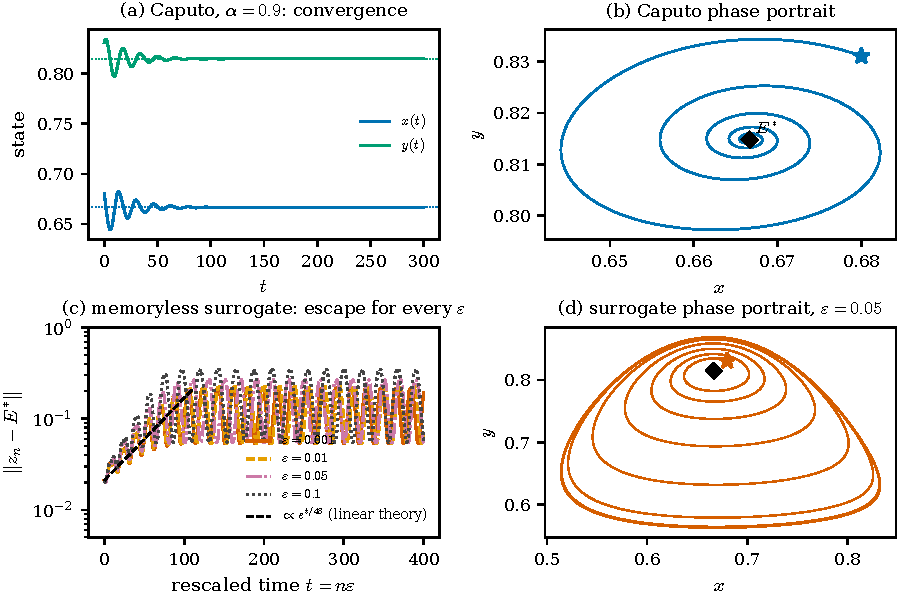
\includegraphics[width=0.85\textwidth]{figA_caputo_vs_surrogate.pdf}
\caption{{Theorem} 
~\ref{thm:inversion} at the benchmark $(A,\alpha)=(3/10,9/10)$ from $1.02\,E^{*}$.
(\textbf{a}) Caputo time series and (\textbf{b}) phase portrait (PECE, $T=300$, $n=3000$).
(\textbf{c}) The memoryless map escapes for every $\varepsilon$ shown along the
linear-theory slope $e^{t/48}$ in the rescaled time $t=n\varepsilon$. (\textbf{d}) Its orbit
at $\varepsilon=0.05$.{{Illustration; the theorem covers every $\varepsilon>0$.}}}
\label{fig:caputovssurr}
\end{figure}

\subsubsection*{{Other Initial Conditions}}

\textls[-15]{The figures above start from one perturbed initial condition. Figure~\ref{fig:ics} repeats
the benchmark experiment (PECE, $T=300$, $n=3000$) from six initial conditions,
$1.02\,E^{*}$, $1.30\,E^{*}$, $(0.95,0.30)$, $(0.45,1.40)$, $(1.20,0.60)$ above the carrying
capacity, and $(0.25,0.60)$ inside the extinction strip $x_{0}<A$. At $\alpha=0.9$
every trajectory outside the strip approaches $E^{*}$, algebraically slowly in the tail as
the Mittag-Leffler theory predicts, and the strip trajectory goes extinct as
Theorem~\ref{thm:extinction} requires; at $\alpha=0.99$ the trajectories started near
$E^{*}$ depart from it while those started far away are still in transit at $T=300$, about
which no asymptotic claim \linebreak  is made.}

\begin{figure}[H]
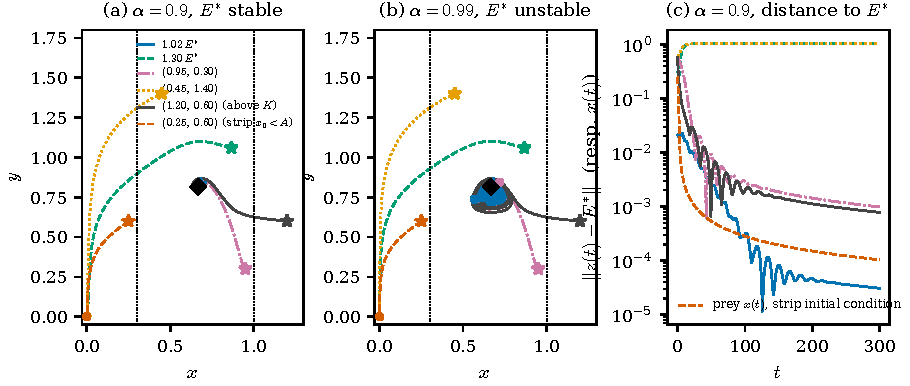
\includegraphics[width=\textwidth]{fig11_initial_conditions.pdf}
\caption{\textls[-15]{Six initial conditions at the benchmark $A=3/10$, listed in the legend of (a), at
(\textbf{a}) $\alpha=0.9$ and (\textbf{b}) $\alpha=0.99$: stars mark initial states, dots
the states at $T$, the diamond $E^{*}$, dotted lines $x=A$ and $x=K$. (\textbf{c}) Distance
to $E^{*}$ at $\alpha=0.9$, and the prey biomass of the strip trajectory.}
{{}}}
\label{fig:ics}
\end{figure}

\subsection{History-Retaining Schemes on the Benchmark}\label{sec:num-schemes}

Figure~\ref{fig:schemes} corroborates Theorem~\ref{thm:gl-implicit} and
Propositions~\ref{prop:gl-explicit} and \ref{prop:onestep} at the benchmark eigenvalue
$\upmu=\tfrac1{48}+\tfrac{i}{2}\sqrt{2107/2880}$ and $\alpha=0.9$, for which
$|\arg\upmu|=1.5221>\alpha\pi/2=1.4137$ and $\Real\upmu>0$. Panel (a) shows the sets
described in Remark~\ref{rem:dichotomy} (i) in one plane; the ray in the direction of
$\arg\upmu$ is the set of all scaled eigenvalues over all step sizes. Panel (b) shows the
implicit scheme on the test equation at $h=0.1$, $1$, $10$, and $100$: all four runs
follow the exact solution and the algebraic asymptote of Theorem~\ref{thm:gl-implicit} (a),
and the normalized tail $y_{n}\upmu\,\Gamma(1-\alpha)\,t_{n}^{\alpha}$ equals $-1.000$ to
three decimals at the end of every run. Panel (c) is the verdict as a function of the step:
the memoryless map amplifies for every $\varepsilon$, the implicit scheme damps for every
$h$, and the explicit scheme damps exactly for $h<h_{0}=0.505$. Panel (d) is the nonlinear
benchmark from $1.02\,E^{*}$: PECE and both Gr\"unwald--Letnikov schemes are within
$3\times10^{-5}$ of $E^{*}$ at $T=300$, at step sizes from $0.05$ to $1$, while the
memoryless orbits saturate at a distance of order $10^{-1}$.

\begin{figure}[H]
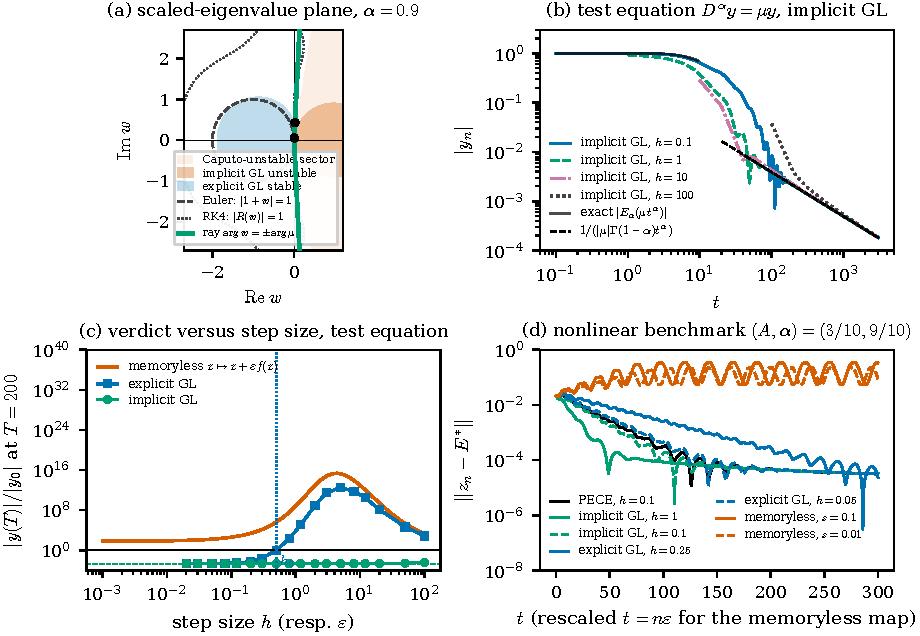
\includegraphics[width=\textwidth]{fig09_schemes_dichotomy.pdf}
\caption{{The} 
 dichotomy of Section~\ref{sec:faithful} at the benchmark eigenvalue, $\alpha=0.9$.
(\textbf{a}) Scaled-eigenvalue plane: the stability sets of Remark~\ref{rem:dichotomy} (i)
and the ray of scaled benchmark eigenvalues. (\textbf{b}) Implicit scheme on the test
equation at four step sizes, with the exact solution and asymptote. (\textbf{c}) Amplitude
at $T=200$ against the step size. (\textbf{d}) Nonlinear benchmark. {{(\textbf{a}) analytic;
(\textbf{b})--(\textbf{d}) corroboration.}}}
\label{fig:schemes}
\end{figure}

\subsection{Continuation and Regime Maps}\label{sec:num-maps}


{Figure}~\ref{fig:continuation} gives the one-parameter view, the branch with its exact
breakpoints and the displacement of the stability switch by the fractional order, and
Figure~\ref{fig:regimemap} gives the two-parameter view: finite-horizon endpoints laid under the
exact atlas boundary, never asymptotic claims. Each cell of the map is classified literally
at $T=200$: near $E^{*}$ if $\|z(T)-E^{*}\|<10^{-2}$, low prey if $x(T)<10^{-3}$, otherwise
transient. The extinction-strip theorem does not apply to these runs, whose initial prey
level $1.05\,x^{*}=0.7$ exceeds every $A$ shown.

\begin{figure}[H]
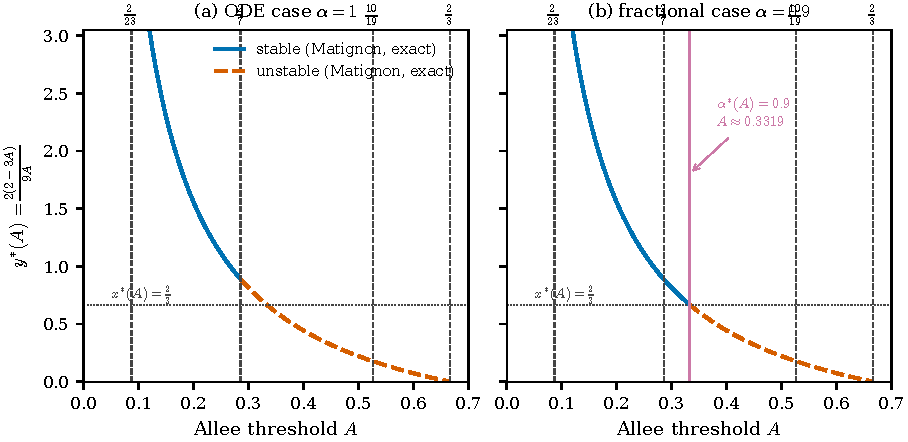
\includegraphics[width=\textwidth]{figC_continuation_A.pdf}
\caption{\textls[-15]{l{The}
 coexistence branch $y^{*}(A)=2(2-3A)/(9A)$, $x^{*}=2/3$, with exact stability
coding from the rational $T(A)$, $D(A)$: solid Matignon-stable, dashed Matignon-unstable.
(\textbf{a}) $\alpha=1$: the switch is at $A=2/7$. (\textbf{b}) $\alpha=0.9$: it moves to
the solution of $\alpha^{*}(A)=0.9$, $A\approx0.3319$. {{Analytic content.}}}}
\label{fig:continuation}
\end{figure}
\unskip
\begin{figure}[H]
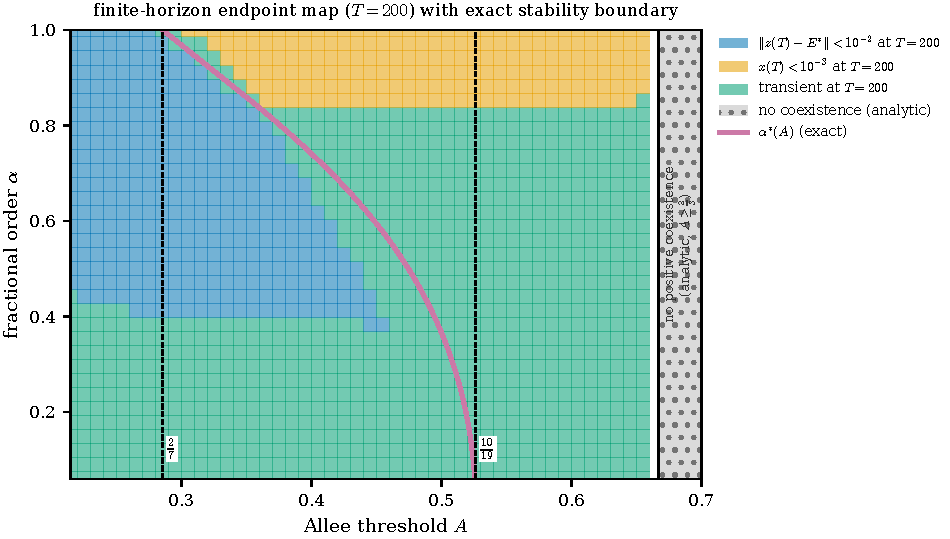
\includegraphics[width=0.85\textwidth]{figD_regime_map.pdf}
\caption{Finite-horizon endpoint map: one PECE run per cell from $1.05\,E^{*}(A)$, $T=200$,
\linebreak  $n=1600$, classified at $T$ as near $E^{*}$ (blue), low prey (orange), or transient (green);
grey: no coexistence equilibrium. The curve $\alpha^{*}(A)$ and the breakpoints are exact.
Transient cells near the curve are the horizon effect of Table~\ref{tab:convergence}.
{{Finite-horizon diagnostics; exact overlay.}}}
\label{fig:regimemap}
\end{figure}

\subsection{Beyond the Benchmark}\label{sec:num-beyond}

Theorem~\ref{thm:general-atlas} and Corollary~\ref{cor:open} say that the benchmark atlas
is one instance of an open phenomenon. {Figure}~\ref{fig:beyond} and
Table~\ref{tab:beyond} exhibits it on two further parameter sets chosen to have no rational
structure: Set II, with generic rational coefficients $r=1$, $a=5/2$, $h=3/2$, $e=11/20$,
$m=1/2$ ($q=4/5$), and Set III, with irrational coefficients $r=\sqrt2$, $a=1+\sqrt3$,
$h=\pi/4$, $e=1/\sqrt3$, $m=1/\sqrt2$ ($q=0.6919\ldots$), both with $K=1$. In both,
$c_{T}<0$ and the six-row atlas appears with its own breakpoints; for Set III every
breakpoint is a certified Arb enclosure of width below $10^{-6}$, computed from
Equation~\eqref{eq:affine} with the same arithmetic as the proof objects. Inside the wedge of Set II,
at $(A,\alpha)=(\setIIA,\setIIalpha)$ where $\alpha^{*}(A)=\setIIalphastar$ and
$\Real\upmu=\setIIReMu>0$, PECE ($h=0.1$) and the implicit Gr\"unwald--Letnikov scheme
($h=0.5$) converge to $E^{*}$ while the memoryless map escapes at $\varepsilon=0.1$ and
$0.01$ (Figure~\ref{fig:beyond}c): the dichotomy is not a property of the benchmark.

\begin{figure}[H]
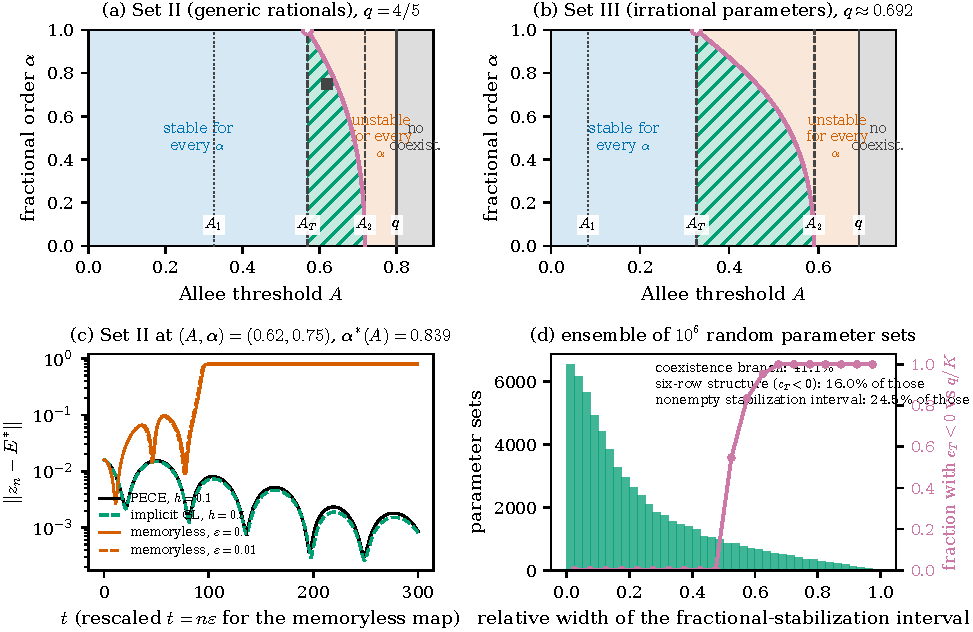
\includegraphics[width=0.85\textwidth]{fig10_beyond_benchmark.pdf}
\caption{{The atlas} 
 beyond the benchmark. (\textbf{a}) Set~II and (\textbf{b}) Set~III, breakpoints
in Table~\ref{tab:beyond}; the square in (\textbf{a}) is the point of (\textbf{c}). (\textbf{c}) Set~II inside
its wedge: PECE, implicit scheme, memoryless map. \linebreak  (\textbf{d}) Ensemble of $\ensembleN$
random parameter sets: width of the stabilization interval, and fraction with $c_{T}<0$
against $q/K$. {{(\textbf{a}), (\textbf{b}) analytic; (\textbf{c},\textbf{d}) corroboration.}}}
\label{fig:beyond}
\end{figure}

How common is the structure? In an ensemble of $\ensembleN$ parameter sets drawn
log-uniformly from $r,a\in[0.1,10]$, $h\in[0.01,10]$, $e\in[0.05,1]$, $m\in[0.01,5]$ with
$K=1$, a coexistence branch ($ea>mh$, $q<K$) exists for $\ensembleCoexistPct\%$ of the
sets; of these, $\ensembleSixRowPct\%$ satisfy $c_{T}<0$ and therefore carry the full
six-row atlas with $\alpha^{*}$ ranging over all of $(0,1)$, and $\ensembleWedgePct\%$ have
a nonempty fractional-stabilization interval (the difference being sets with $c_{T}\ge0$,
where $\alpha^{*}<1$ on the interval, Theorem~\ref{thm:general-atlas} (d)). Among the
six-row sets the relative width $(A_{2}-A_{T})/q$ of the stabilization interval has median
$\ensembleWidthMedian$ and interquartile range
$[\ensembleWidthQa,\ensembleWidthQb]$, and the fraction with $c_{T}<0$ rises steeply with
$q/K$ and reaches one for $q/K\ge2/3$, as Corollary~\ref{cor:open} predicts. These are
statistics over an arbitrary sampling measure and carry no ecological weight; their content
is that the phenomenon occupies a set of parameters with positive measure, not a
fine-tuned point.



\begin{table}[H]
\caption{Breakpoints of the atlas for the three parameter sets, from Equation~\eqref{eq:affine}.
Exact rationals where the data are rational; otherwise Arb enclosures, printed with outward
rounding to six decimals.\label{tab:beyond}}
%% generated by figures/src/fig10_beyond_benchmark.py; do not edit by hand
\small
\begin{tabularx}{\textwidth}{cCCC}
\toprule
 & \textbf{Set I (benchmark)} & \textbf{Set II} & \textbf{Set III} \\
\midrule
$q$ & $2/3$ & $4/5$ & $[0.691892,\,0.691893]$ \\
$c_{T}$ & $-1/4$ & $-108/275$ & $[-0.269381,\,-0.269380]$ \\
$A_{1}$ (zero of $\Delta$) & $2/23$ & $[0.325837,\,0.325838]$ & $[0.083007,\,0.083008]$ \\
$A_{T}$ (zero of $T$) & $2/7$ & $54/95$ & $[0.326494,\,0.326495]$ \\
$A_{2}$ (zero of $\Delta$) & $10/19$ & $[0.718094,\,0.718095]$ & $[0.590981,\,0.590982]$ \\
arithmetic & exact rational & exact rational; Arb for the zeros of $\Delta$ & Arb enclosures throughout \\
\bottomrule
\end{tabularx}

\end{table}


%=====================================================================
\section{Discussion and Conclusions}\label{sec:discussion}
%=====================================================================

\subsection{{What Is New, and What Is for Completeness}
}

The new mathematics is in Sections~\ref{sec:general-atlas} and \ref{sec:inversion}: the
affine structure of $(T,D)$ in $1/A$, which turns the benchmark atlas into an instance of a
theorem valid on an open set of parameters, and the discretization dichotomy, which
separates memoryless one-step maps from history-retaining schemes by a structural property
on an exactly described region. The reduction in Section~\ref{sec:atlas} is what both rest
on. The global results of Section~\ref{sec:global} are standard in method and included for
completeness, and Proposition~\ref{prop:basins} states what they leave open. The proof
objects and the numerics are evidence about constants and trajectories, not part of any
proof.

\subsection{What the Dichotomy Means for Method Choice}

On the fractional-stabilization region, an explicit memoryless map does not merely lose
accuracy; it returns the opposite qualitative answer at every step size, and so does every
consistent memoryless one-step method at all sufficiently small steps. The remedy is not a
smaller step but a scheme that carries the history: the implicit Gr\"unwald--Letnikov scheme
returns the correct verdict at every step size and reproduces the exact algebraic tail, the
explicit one at every sufficiently small step, and the predictor--corrector method in
practice. Near the critical order, every method is slow, for the reason quantified in
Table~\ref{tab:convergence}, and a finite-horizon classification there is undecided by
nature rather than by defect.

\subsection{Which Conclusions Admit an Ecological Reading, and Which Do Not}

The paper is mathematical, and the benchmark is not calibrated
(Definition~\ref{def:benchmark}); the rational breakpoints carry no ecological meaning. Four
statements do have a reading in the model's own terms. (i) The Allee threshold $A$ is a
genuine extinction threshold for the prey: below it, the prey goes extinct with a
Mittag-Leffler envelope whatever the predator does, and on the predator-free face the
threshold is sharp (Proposition~\ref{prop:basins}). (ii) Coexistence requires
$A<q<K$: the prey level $q$ at which the predator breaks even must lie between the Allee
threshold and the carrying capacity. (iii) Fractional stabilization arises under
$c_{T}<0$, which holds whenever $q/K\ge2/3$ and for small handling time reduces to $q/K>1/2$
(Corollary~\ref{cor:open}): a predator whose break-even prey level is high relative to the
carrying capacity is the structural setting in which memory can stabilize coexistence that
classical linearization rejects. (iv) The order $\alpha$ is read here, as in the modeling
literature \cite{Ahmed2007,Du2013,Saeedian2017}, as a phenomenological summary of history
dependence of past densities acting on present demographic rates through delayed or
cumulative effects, and not as a measured quantity. Whether a given population has
$\alpha<1$ in this sense, and which value is an empirical question we do not address. What
the atlas shows is that the qualitative outcome depends on $\alpha$ discontinuously at
$\alpha^{*}(A)$, so a modeling decision about memory is not a matter of fine-tuning. An
applied reading of any specific number in this paper would require fitting $r,K,a,h,e,m$ and
$\alpha$ to data, which we have not done.

\subsection{Evidence Boundaries}

Four categories are kept apart throughout, because blurring them is the failure mode of
computer-assisted work. {{Theorem}}: Sections~\ref{sec:atlas}--\ref{sec:global} and
Appendix~\ref{app:proofs}. {{Certified computation}}: the proof objects of
Section~\ref{sec:certificates} and the enclosures of Table~\ref{tab:beyond}, exactly where the
claim is algebraic and enclosed otherwise. {{Numerical corroboration}}:
Section~\ref{sec:numerics}. {{Open}}: the items below. A theorem may also carry a partial
machine audit of selected constants; such an audit is additional evidence and does not
change the analytic status of the theorem.

\subsection{Open Problems}

The boundary between the basins of $E_{0}$ and $E^{*}$, and any global asymptotic stability
statement for $E^{*}$, are not addressed (Proposition~\ref{prop:basins}). Nothing is
asserted about the nonlinear dynamics at the critical boundaries of
Proposition~\ref{prop:critical}. A small-step verdict-faithfulness statement for the
predictor--corrector method, analogous to Proposition~\ref{prop:gl-explicit}, is not proved
here. Certification over a parameter box that straddles an algebraic or Matignon boundary
returns {{undecided}} by design; a compact wide-box certificate returning a verdict with an
explicit boundary decomposition remains to be built. Periodic orbits, chaotic dynamics, and
control of Equation~\eqref{eq:model} are outside the scope of this paper.

\subsection{Reproducibility}

The LaTeX source, the figure and table generation scripts with their machine-readable
output data, the proof objects with a completeness-checked SHA-256 manifest, the two
checkers, the symbolic verification script, and a test suite with negative fixtures are
available from the corresponding author on request; two commands re-derive every object and
rebuild every figure, table, and the paper.

\subsection{Conclusions}

For a strong-Allee, Holling type-II predator--prey system under a commensurate Caputo
derivative, the local stability of the coexistence equilibrium reduces exactly to two scalars
that are affine in the reciprocal Allee threshold. Under one explicit open inequality every
parameter set carries the same six-row stability atlas with a strictly decreasing critical
order, and the benchmark atlas with rational breakpoints is one instance of it. The atlas
contains a region where memory stabilizes an equilibrium that classical linearization
rejects, and on that region discretization splits along a structural line: memoryless
one-step maps invert the verdict for every step size in the Euler case and for all small
steps in general, while the Gr\"unwald--Letnikov schemes, which retain the history, return
it, for every step size in the implicit case and for all small steps in the explicit one.
Positivity, a sharp-on-face extinction strip, a uniform ultimate bound, and global existence
complete the picture; selected constants are audited by machine-checkable objects, and the
numerical evidence extends to two further parameter sets and to a random ensemble.


%=====================================================================
\authorcontributions{\textls[-15]{Conceptualization, I.A. and T.N.A.; methodology, I.A. and T.N.A.; formal
analysis, I.A. and T.N.A.; verification software, I.A.; writing---original
draft, I.A.; writing---review and editing, I.A. and T.N.A. All authors have read and agreed to the published version of the manuscript}}

\funding{This research received no external {funding.} }

%\institutionalreview{Not applicable.}

%\informedconsent{Not applicable.}

\dataavailability{The original contributions presented in this study are
included in the article. Further inquiries can be directed to the corresponding author.
%AUTHOR :  We confirm to remove this section   
%MDPI: “Not applicable” is only used for review papers or articles in which no new data were created. Please state it according to the data availability status; for example, if the data are contained within the article, state “The original contributions presented in this study are included in the article. Further inquiries can be directed to the corresponding author(s).” Please refer to the complete guidelines at https://www.mdpi.com/ethics#_bookmark21.
}

\acknowledgments{\textls[-25]{{The authors are thankful to the Deanship of Graduate Studies and Scientific Research at University of Bisha for supporting this work through the Fast-Track Research Support Program.}} 

% Author: we need to thanks univeristy in acknowedgment section, Please keep it 
%MDPI: Attention Assigned Editor: please confirm whether the funding information in the Acknowledgments section should be moved to the Funding section.
}

\conflictsofinterest{The authors declare no conflicts of interest.}


\appendixtitles{no} % Leave argument "no" if all appendix headings stay EMPTY (then no dot is printed after "Appendix A"). If the appendix sections contain a heading then change the argument to "yes".
\appendixstart
\appendix
\section[\appendixname~\thesection]{Proofs for Section~\ref{sec:faithful}}\label{app:proofs}

%=====================================================================

%=====================================================================

\textls[-15]{Throughout, $(1-\xi)^{\beta}:=\exp(\beta\operatorname{Log}(1-\xi))$ with the principal
logarithm. It is analytic on $\Cn\setminus[1,\infty)$, hence, on the open unit disc
$\mathbb{D}$, and continuous on $\overline{\mathbb{D}}\setminus\{1\}$. For
$\xi\in\overline{\mathbb{D}}\setminus\{1\}$ the point $1-\xi$ lies in the closed disc
$|w-1|\le1$ punctured at $0$, so $|\operatorname{Arg}(1-\xi)|<\pi/2$ and}
\begin{equation}\label{eq:lens}
  (1-\xi)^{\alpha}\in S_{\alpha}:=\{w\neq0:\ |\operatorname{Arg}w|<\alpha\pi/2\},
  \qquad |(1-\xi)^{\alpha}|\le2^{\alpha}.
\end{equation}

We use two facts from singularity analysis \cite[Thms.~VI.1 and VI.3]{FlajoletSedgewick2009}.
A \emph{$\Delta$-domain} at $1$ is a set
$\{\xi:|\xi|<1+\eta,\ \xi\neq1,\ |\operatorname{Arg}(\xi-1)|>\varphi\}$ with $\eta>0$ and
$0<\varphi<\pi/2$. If $G(\xi)=\sum g_{n}\xi^{n}$ is analytic in a $\Delta$-domain and
$G(\xi)=c\,(1-\xi)^{-\beta}+O(|1-\xi|^{-\gamma})$ as $\xi\to1$ there, with
$\beta\notin\{0,-1,-2,\dots\}$ and $\gamma<\beta$, then
\begin{equation}\label{eq:transfer}
  g_{n}=\frac{c}{\Gamma(\beta)}\,n^{\beta-1}+O(n^{\gamma-1}).
\end{equation}

\begin{proof}[Proof of Theorem~\ref{thm:gl-implicit}]
\textls[-15]{Let $u_{n}=y_{n}-y_{0}$, so $u_{0}=0$, and write the scheme for $n\ge1$ as
$\sum_{j=0}^{n}\omega_{j}u_{n-j}=z\,y_{n}=z(u_{n}+y_{0})$ with $z=h^{\alpha}\upmu$. The
coefficient of $u_{n}$ is $\omega_{0}-z=1-z$, so the scheme is well defined iff $z\neq1$;
under either hypothesis $z$ is not a positive real number in case (a), and $z\neq1$ is
assumed in case (b). Let $U(\xi)=\sum_{n\ge0}u_{n}\xi^{n}$ and
\linebreak  $Y(\xi)=\sum_{n\ge0}y_{n}\xi^{n}=U(\xi)+y_{0}/(1-\xi)$ as formal power series. Multiplying
the scheme by $\xi^{n}$ and summing over $n\ge1$ (the $n=0$ term of the convolution is
$\omega_{0}u_{0}=0$, so the sum may start at $n=0$ on the left) gives
$(1-\xi)^{\alpha}U(\xi)=z\bigl(Y(\xi)-y_{0}\bigr)=zU(\xi)+zy_{0}\xi/(1-\xi)$, hence}
\begin{equation}\label{eq:Yimplicit}
  Y(\xi)\;=\;y_{0}\,\frac{(1-\xi)^{\alpha-1}-z}{(1-\xi)^{\alpha}-z}
  \;=:\;y_{0}\,\frac{N(\xi)}{g(\xi)} .
\end{equation}

The identity holds as a formal power series, and both sides are analytic wherever $g\neq0$ in
$\mathbb{D}$, so the coefficients of the analytic function on the right are the $y_{n}$.

{(a) Let}
 $|\arg\upmu|>\alpha\pi/2$, so $z\notin\overline{S_{\alpha}}$. By Equation~\eqref{eq:lens},
$g(\xi)=(1-\xi)^{\alpha}-z\neq0$ on $\overline{\mathbb{D}}\setminus\{1\}$, and $g(1)=-z\neq0$.
Since $(1-\xi)^{\alpha}\to0$ as $\xi\to1$ in $\Cn\setminus[1,\infty)$, $g$ is bounded away from
zero on a neighborhood of $1$ in that slit plane; on the rest of $\overline{\mathbb{D}}$, a
compact set on which $g$ is continuous and nonvanishing, $g$ is bounded away from zero as
well, and by uniform continuity the same holds on $\{|\xi|\le1+\eta\}\setminus[1,\infty)$ for
some $\eta>0$. Hence, $Y$ is analytic in a $\Delta$-domain. As $\xi\to1$,
$1/g(\xi)=-z^{-1}\bigl(1-(1-\xi)^{\alpha}/z\bigr)^{-1}=-z^{-1}\bigl(1+O(|1-\xi|^{\alpha})\bigr)$,
so
\begin{align*}
  Y(\xi)&=-\frac{y_{0}}{z}(1-\xi)^{\alpha-1}+O\bigl(|1-\xi|^{2\alpha-1}\bigr)+O(1)\\
        &=-\frac{y_{0}}{z}(1-\xi)^{-(1-\alpha)}+O\bigl(|1-\xi|^{-\gamma}\bigr),
  \qquad \gamma=\max\{1-2\alpha,0\}<1-\alpha .
\end{align*}

By Equation~\eqref{eq:transfer} with $\beta=1-\alpha\in(0,1)$,
\[
  y_{n}=-\frac{y_{0}}{z\,\Gamma(1-\alpha)}\,n^{-\alpha}+O\bigl(n^{\gamma-1}\bigr),
  \qquad \gamma-1<-\alpha ,
\]
and $z\,n^{\alpha}=\upmu\,(nh)^{\alpha}=\upmu\,t_{n}^{\alpha}$ gives the stated asymptotics; in
particular $y_{n}\to0$. The exact solution has the same leading term
\cite[Ch.~1]{Podlubny1999}.

{(b) Let} $|\arg\upmu|<\alpha\pi/2$ and $0<h<h_{1}$. Then $|\operatorname{Arg}z|=|\arg\upmu|<\alpha\pi/2$,
so $z^{1/\alpha}:=\exp(\operatorname{Log}z/\alpha)$ satisfies
$|\operatorname{Arg}z^{1/\alpha}|<\pi/2$ and $(z^{1/\alpha})^{\alpha}=z$. Put
$\xi^{*}=1-z^{1/\alpha}$. Then, $|\xi^{*}|<1$ iff
$|z|^{2/\alpha}<2|z|^{1/\alpha}\cos(\arg\upmu/\alpha)$, i.e.,\ iff
$h|\upmu|^{1/\alpha}<2\cos(\arg\upmu/\alpha)$, which is $h<h_{1}$. The map $w\mapsto w^{\alpha}$
is injective on the right half-plane, so $\xi^{*}$ is the only zero of $g$ in
$\overline{\mathbb{D}}$, and it is simple because $g'(\xi^{*})=-\alpha(1-\xi^{*})^{\alpha-1}\neq0$.
The numerator at the pole is
$N(\xi^{*})=z^{(\alpha-1)/\alpha}-z=z\,(z^{-1/\alpha}-1)$, which vanishes only if
$z^{-1/\alpha}=1$, i.e.,\ $z=1$; this is excluded. Hence $Y=c/(1-\xi/\xi^{*})+\widetilde Y$
with $c\neq0$ and $\widetilde Y$ analytic in $\mathbb{D}$, with the same $\Delta$-domain
analyticity and the same expansion at $1$ as in (a); so
$y_{n}=c\,(\xi^{*})^{-n}+O(n^{-\alpha})$ and $|y_{n}|\to\infty$ like $|\xi^{*}|^{-n}$.

The last sentence of the theorem is (a) applied to $\upmu_{\pm}$, whose arguments exceed
$\alpha\pi/2$ on $\mathcal{W}$, together with Theorem~\ref{thm:inversion}.
\end{proof}

\begin{proof}[Proof of Proposition~\ref{prop:gl-explicit}]
\textls[-35]{With $u_{n}$, $U$, $Y$, and $z$ as above, the explicit scheme reads
$\sum_{j=0}^{n}\omega_{j}u_{n-j}=z\,y_{n-1}$ for $n\ge1$, and summing gives
$(1-\xi)^{\alpha}U(\xi)=z\xi Y(\xi)=z\xi U(\xi)+z\xi y_{0}/(1-\xi)$, hence}
\begin{equation}\label{eq:Yexplicit}
  Y(\xi)=y_{0}\,\frac{(1-\xi)^{\alpha-1}}{g_{e}(\xi)},\qquad g_{e}(\xi):=(1-\xi)^{\alpha}-z\xi .
\end{equation}

The scheme is always well defined ($\omega_{0}=1$). Its stability set is
$\{z:\ g_{e}\text{ has no zero in }\overline{\mathbb{D}}\}$, and $g_{e}(e^{i\theta})=0$ iff
$z=(1-e^{i\theta})^{\alpha}e^{-i\theta}$, which is the boundary locus in the statement.

\textls[-15]{{{Localization.}
} If $\xi\in\overline{\mathbb{D}}$ and $g_{e}(\xi)=0$ then
$|1-\xi|^{\alpha}=|z||\xi|\le|z|$, so $|1-\xi|\le|z|^{1/\alpha}$: for small $|z|$ every zero
in $\overline{\mathbb{D}}$ lies near $1$; once $|1-\xi|\le1/2$ we have $|\xi|\ge1/2$ and
$|\operatorname{Arg}\xi|\le\tfrac{\pi}{2}|\sin\operatorname{Arg}\xi|
=\tfrac{\pi}{2}\,|\Imag\xi|/|\xi|\le\pi|1-\xi|\le\delta(z):=\pi|z|^{1/\alpha}\to0$. Writing
$1-\xi=\rho e^{i\varphi}$ with $|\varphi|<\pi/2$ and taking arguments in
$(1-\xi)^{\alpha}=z\xi$ gives $\alpha\varphi\equiv\operatorname{Arg}z+\operatorname{Arg}\xi
\pmod{2\pi}$. Both $|\alpha\varphi|<\alpha\pi/2<\pi/2$ and $|\operatorname{Arg}\xi|\le\delta$,
so for $\delta<\pi/2$ the congruence is an equality and}
\begin{equation}\label{eq:argbound}
  |\operatorname{Arg}z|\;\le\;\alpha\pi/2+\delta(z).
\end{equation}

{{Case} $|\arg\upmu|>\alpha\pi/2$.} Since $\operatorname{Arg}z=\arg\upmu$, choose $h_{0}$ so that
$\delta(h^{\alpha}\upmu)<|\arg\upmu|-\alpha\pi/2$ for $h<h_{0}$. Then Equation~\eqref{eq:argbound} fails
for every $\xi\in\overline{\mathbb{D}}$, so $g_{e}$ has no zero there; $g_{e}(1)=-z\neq0$, and
as in part (a) above, $Y$ is analytic in a $\Delta$-domain with
$1/g_{e}(\xi)=-z^{-1}\bigl(1+O(|1-\xi|^{\alpha})\bigr)$ as $\xi\to1$. Hence,
$Y=-(y_{0}/z)(1-\xi)^{\alpha-1}+O(|1-\xi|^{2\alpha-1})$, and Equation~\eqref{eq:transfer} gives
$y_{n}=-y_{0}\,(\upmu\Gamma(1-\alpha)t_{n}^{\alpha})^{-1}(1+o(1))\to0$: the explicit scheme,
too, reproduces the exact tail whenever it is stable.

{{Case} $|\arg\upmu|<\alpha\pi/2$.} Let $\xi_{0}=1-z^{1/\alpha}$, the zero of
$g(\xi)=(1-\xi)^{\alpha}-z$, and put $\kappa=\tfrac12\cos(\arg\upmu/\alpha)\in(0,\tfrac12]$ and
$\Gamma_{z}=\{\xi:|\xi-\xi_{0}|=\kappa|z|^{1/\alpha}\}$. On $\Gamma_{z}$, $1-\xi=z^{1/\alpha}
(1+\kappa e^{i\theta})$, so $g(\xi)=z\bigl[(1+\kappa e^{i\theta})^{\alpha}-1\bigr]$ and
$|g|\ge c(\alpha,\kappa)|z|$ with $c(\alpha,\kappa)=\min_{\theta}|(1+\kappa e^{i\theta})^{\alpha}-1|>0$
(the minimum is positive because $(1+\kappa e^{i\theta})^{\alpha}=1$ forces
$1+\kappa e^{i\theta}=1$). Also $|g_{e}-g|=|z||1-\xi|\le(1+\kappa)|z|^{1+1/\alpha}$ on
$\Gamma_{z}$, which is smaller than $c(\alpha,\kappa)|z|$ once $|z|^{1/\alpha}<c/(1+\kappa)$.
By Rouch\'e's theorem, $g_{e}$ has exactly one zero $\xi_{e}$ inside $\Gamma_{z}$. The circle
lies in $\mathbb{D}$: with $w=1-\xi$, $|\xi|<1$ iff $|w|^{2}<2\Real w$, and on $\Gamma_{z}$,
$\Real w\ge|z|^{1/\alpha}(\cos(\arg\upmu/\alpha)-\kappa)=\kappa|z|^{1/\alpha}$ while
$|w|^{2}\le(1+\kappa)^{2}|z|^{2/\alpha}$, so the inequality holds once
$|z|^{1/\alpha}<2\kappa/(1+\kappa)^{2}$. The zero is simple for small $|z|$, because
$g_{e}'(\xi)=-\alpha(1-\xi)^{\alpha-1}-z$ and $|\alpha(1-\xi)^{\alpha-1}|\asymp|z|^{(\alpha-1)/\alpha}
\to\infty$ while $|z|\to0$. The numerator $(1-\xi)^{\alpha-1}$ in Equation~\eqref{eq:Yexplicit} does
not vanish, so $Y$ has a simple pole with nonzero residue at $\xi_{e}\in\mathbb{D}$ and
$|y_{n}|\to\infty$ like $|\xi_{e}|^{-n}$. Taking $h_{0}$ so that $|z|=h^{\alpha}|\upmu|$
satisfies the two smallness conditions for $h<h_{0}$ completes the proof.
\end{proof}

\begin{proof}[Proof of Proposition~\ref{prop:onestep}]
$|R(\varepsilon\upmu)|^{2}=|1+\varepsilon\upmu+O(\varepsilon^{2})|^{2}
=1+2\varepsilon\Real\upmu+O(\varepsilon^{2})$, which exceeds $1$ for all sufficiently small
$\varepsilon>0$ when $\Real\upmu>0$. For $R(w)=1+w$ the $O(\varepsilon^{2})$ term is
$\varepsilon^{2}|\upmu|^{2}\ge0$, which is Lemma~\ref{lem:multiplier}.
\end{proof}

%=====================================================================
\begin{adjustwidth}{-\extralength}{0cm}
%} % If the paper is ``preprints'', please uncomment this parenthesis.
%\printendnotes[custom] % Un-comment to print a list of endnotes

\reftitle{References}
\begin{thebibliography}{999}

\bibitem{Matignon1996}
{Matignon, D.} 
 Stability results for fractional differential equations with applications to control processing. In Proceedings of the Computational Engineering in Systems Applications, Lille, France, 9--12 July 1996; pp. 963--968.

\bibitem{Ahmed2007}
Ahmed, E.; El-Sayed, A.M.A.; El-Saka, H.A.A. Equilibrium points, stability and numerical solutions of fractional-order predator--prey and rabies models. \emph{J. Math. Anal. Appl.} \textbf{2007}, \emph{325}, 542--553. \url{https://doi.org/10.1016/j.jmaa.2006.01.087}.

\bibitem{Saha2026}
Saha, A.; Pal, D.; Kesh, D.; Mukherjee, D. A fractional-order commensurate and incommensurate study on predator-prey system with Allee in predator and fear effect. \emph{Fract. Calc. Appl. Anal.} \textbf{2026}, \emph{29}, 1486--1515. \url{https://doi.org/10.1007/s13540-026-00515-8}.

\bibitem{Ramesh2025}
\textls[-35]{Ramesh, K.; Ranjith Kumar, G.; Khan, A.; Abdeljawad, T. Analysis of the stability of a predator-prey model including the memory effect, double Allee effect and Holling type-I functional response. \emph{PLoS ONE} \textbf{2025}, \emph{20}, e0305179. \url{https://doi.org/10.1371/journal.pone.0305179}.}

\bibitem{WangHan2025}
Wang, Q.; Han, R. Dynamics of fractional order predator prey models with refuge and Allee effect in prey: With and without time delay. \emph{Qual. Theory Dyn. Syst.} \textbf{2025}, \emph{24}, 49. \url{https://doi.org/10.1007/s12346-024-01212-8}.

\bibitem{Baghel2026}
Baghel, R.S. Hopf bifurcation and stability in a fractional-order age-structured predator-prey model with Allee effect and dual delays. \emph{Chaos Solitons Fractals} \textbf{2026}, \emph{205}, 117880. \url{https://doi.org/10.1016/j.chaos.2026.117880}.


\bibitem{Mondal2025}
Mondal, C.; Mondal, R.; Kesh, D.; Mukherjee, D. Dynamics of predator-prey system with the consequences of double Allee effect in prey population. \emph{J. Biol. Phys.} \textbf{2025}, \emph{51}, 5. \url{https://doi.org/10.1007/s10867-025-09670-0}.


\bibitem{Rahmi2026}
Rahmi, E.; Anggriani, N.; Panigoro, H.S.; Peter, O.J. A fractional-order approach to predator-prey interactions: Modeling fear and disease dynamics with memory effects. \emph{PLoS ONE} \textbf{2026}, \emph{21}, e0339351. \url{https://doi.org/10.1371/journal.pone.0339351}.


\bibitem{Cermak2013}
Čermák, J.; Kisela, T.; Nechvátal, L. Stability regions for linear fractional differential systems and their discretizations. \linebreak  \emph{Appl. Math. Comput.} \textbf{2013}, \emph{219}, 7012--7022. \url{https://doi.org/10.1016/j.amc.2012.12.019}.

\bibitem{CressonSzafranska2017}
Cresson, J.; Szafrańska, A. Discrete and continuous fractional persistence problems---The positivity property and applications. \emph{Commun. Nonlinear Sci. Numer. Simul.} \textbf{2017}, \emph{44}, 424--448. \url{https://doi.org/10.1016/j.cnsns.2016.07.016}.


\bibitem{Elsadany2015}
Elsadany, A.A.; Matouk, A.E. Dynamical behaviors of fractional-order Lotka--Volterra predator--prey model and its discretization. \emph{J. Appl. Math. Comput.} \textbf{2015}, \emph{49}, 269--283. \url{https://doi.org/10.1007/s12190-014-0838-6}.


\bibitem{Mondal2020}
\textls[-35]{Mondal, S.; Biswas, M.; Bairagi, N. Local and global dynamics of a fractional-order predator--prey system with habitat complexity and the corresponding discretized fractional-order system. \emph{J. Appl. Math. Comput.} \textbf{2020}, \emph{63}, 311--340. \url{https://doi.org/10.1007/s12190-020-01319-6}.}

\bibitem{Lubich1986}
Lubich, C. Discretized fractional calculus. \emph{SIAM J. Math. Anal.} \textbf{1986}, \emph{17}, 704--719. \url{https://doi.org/10.1137/0517050}.

\bibitem{Diethelm2002}
Diethelm, K.; Ford, N.J.; Freed, A.D. A predictor-corrector approach for the numerical solution of fractional differential equations. \emph{Nonlinear Dynam} \textbf{2002}, \emph{29}, 3--22.


\bibitem{Garrappa2010}
Garrappa, R. On linear stability of predictor--corrector algorithms for fractional differential equations. \emph{Int. J. Comput. Math.} \linebreak  \textbf{2010}, \emph{87}, 2281--2290. \url{https://doi.org/10.1080/00207160802624331}.

\bibitem{Garrappa2018}
Garrappa, R. Numerical solution of fractional differential equations: A survey and a software tutorial. \emph{Mathematics} \textbf{2018}, \emph{6}, 16. \url{https://doi.org/10.3390/math6020016}.


\bibitem{RauhJaulin2021}
Rauh, A.; Jaulin, L. Novel techniques for a verified simulation of fractional-order differential equations. \emph{Fractal Fract.} \textbf{2021}, \emph{5}, 17. \url{https://doi.org/10.3390/fractalfract5010017}.


\bibitem{Cong2016}
Cong, N.D.; Doan, T.S.; Siegmund, S.; Tuan, H.T. Linearized asymptotic stability for fractional differential equations. \linebreak  {arXiv}  \textbf{2016}, arXiv:1512.04989.

\bibitem{Cong2016b}
Cong, N.D.; Doan, T.S.; Siegmund, S.; Tuan, H.T. An instability theorem for nonlinear fractional differential systems. \linebreak  \emph{Discret. Contin. Dyn. Syst. Ser. B} \textbf{2017}, \emph{22}, 3079--3090.

\bibitem{Diethelm2010}
Diethelm, K. The Analysis of Fractional Differential Equations. In \emph{Lecture Notes in Mathematics 2004}; Springer: Berlin/Heidelberg, Germany, 2010.


\bibitem{Lubich1983}
Lubich, C. Runge--Kutta theory for Volterra and Abel integral equations of the second kind. \emph{Math. Comp.} \textbf{1983}, \emph{41}, 87--102. \url{https://doi.org/10.1090/S0025-5718-1983-0701626-6}.

\bibitem{DiethelmFordFreed2004}
Diethelm, K.; Ford, N.J.; Freed, A.D. Detailed error analysis for a fractional Adams method. \emph{Numer. Algorithms} \textbf{2004}, \emph{36}, 31--52. \url{https://doi.org/10.1023/B:NUMA.0000027736.85078.be}.

\bibitem{Diethelm2007}
Diethelm, K. Smoothness properties of solutions of Caputo-type fractional differential equations. \emph{Fract. Calc. Appl. Anal.} \linebreak  \textbf{2007}, \emph{10}, 151--160.


\bibitem{Luchko2009}
Luchko, Y. Maximum principle for the generalized time-fractional diffusion equation. \emph{J. Math. Anal. Appl.} \textbf{2009}, \emph{351}, 218--223. \url{https://doi.org/10.1016/j.jmaa.2008.10.018}.



\bibitem{LuchkoSuzukiYamamoto2022}
\textls[-15]{Luchko, Y.; Suzuki, A.; Yamamoto, M. On the maximum principle for the multi-term fractional transport equation. \emph{J. Math. Anal. Appl.} \textbf{2022}, \emph{505}, 125579. \url{https://doi.org/10.1016/j.jmaa.2021.125579}.}


\bibitem{AlRefai2012}
Al-Refai, M. On the fractional derivatives at extrema points. \emph{Electron. J. Qual. Theory Differ. Equ.} \textbf{2012}, \emph{55}, 1--5. \linebreak  \url{https://doi.org/10.14232/ejqtde.2012.1.55}.


\bibitem{CongTuan2017}
\textls[-15]{Cong, N.D.; Tuan, H.T. Generation of nonlocal fractional dynamical systems by fractional differential equations. \emph{J. Integral Equ. Appl.} \textbf{2017}, \emph{29}, 585--608.}


\bibitem{Tavazoei2009}
Tavazoei, M.S.; Haeri, M. A proof for non existence of periodic solutions in time invariant fractional order systems. \emph{Automatica} \textbf{2009}, \emph{45}, 1886--1890. \url{https://doi.org/10.1016/j.automatica.2009.04.001}.


\bibitem{Kaslik2012}
Kaslik, E.; Sivasundaram, S. Non-existence of periodic solutions in fractional-order dynamical systems and a remarkable difference between integer and fractional-order derivatives of periodic functions. \emph{Nonlinear Anal. Real. World Appl.} \textbf{2012}, \emph{13}, 1489--1497. \url{https://doi.org/10.1016/j.nonrwa.2011.11.013}.


\bibitem{BaffetHesthaven2017}
Baffet, D.; Hesthaven, J.S. A kernel compression scheme for fractional differential equations. \emph{SIAM J. Numer. Anal.} \linebreak  \textbf{2017}, \emph{55}, 496--520. \url{https://doi.org/10.1137/15M1043960}.


\bibitem{Jiang2017}
Jiang, S.; Zhang, J.; Zhang, Q.; Zhang, Z. Fast evaluation of the Caputo fractional derivative and its applications to fractional diffusion equations. \emph{Commun. Comput. Phys.} \textbf{2017}, \emph{21}, 650--678. \url{https://doi.org/10.4208/cicp.OA-2016-0136}.

\bibitem{Podlubny1999}
Podlubny, I. \emph{Fractional Differential Equations}; Academic Press: San Diego, CA, USA, 1999.



\bibitem{HairerWanner1996}
Hairer, E.; Wanner, G. \emph{Solving Ordinary Differential Equations II. Stiff and Differential-Algebraic Problems}, 2nd ed; Springer Series in Computational Mathematics 14; Springer: Berlin/Heidelberg, Germany, 1996.

\bibitem{FlajoletSedgewick2009}
Flajolet, P.; Sedgewick, R. \emph{Analytic Combinatorics}; Cambridge University Press: Cambridge, UK, 2009.



\bibitem{CarvalhoFehlberg2018}
de Carvalho-Neto, P.M.; Fehlberg Júnior, R. Conditions for the absence of blowing up solutions to fractional differential equations. \emph{Acta Appl. Math.} \textbf{2018}, \emph{154}, 15--29. \url{https://doi.org/10.1007/s10440-017-0130-5}.





\bibitem{Du2013}
Du, M.; Wang, Z.; Hu, H. Measuring memory with the order of fractional derivative. \emph{Sci. Rep.} \textbf{2013}, \emph{3}, 3431. \linebreak  \url{https://doi.org/10.1038/srep03431}.
























\bibitem{Saeedian2017}
Saeedian, M.; Khalighi, M.; Azimi-Tafreshi, N.; Jafari, G.R.; Ausloos, M. Memory effects on epidemic evolution: The susceptible-infected-recovered epidemic model. \emph{Phys. Rev. E} \textbf{2017}, \emph{95}, 022409. \url{https://doi.org/10.1103/PhysRevE.95.022409}.









\end{thebibliography}

\PublishersNote{}
%\isPreprints{}{% This command is only used for ``preprints''.
\end{adjustwidth}
%} % If the paper is ``preprints'', please uncomment this parenthesis.
\end{document}
